% ------------------------------------------------------------------------------
% TYPO3 Version 10 LTS - What's New (French Version)
%
% @license	Creative Commons BY-NC-SA 3.0
% @link		https://typo3.org/help/documentation/whats-new/
% @language	French
% ------------------------------------------------------------------------------

\section{Changements en profondeur}
\begin{frame}[fragile]
	\frametitle{Changements en profondeur}

	\begin{center}\huge{\color{typo3darkgrey}\textbf{Changements en profondeur}}\end{center}
	\begin{center}\large{\textit{Améliorations et nouvelles fonctionnalités pour les intégrateurs et développeurs}}\end{center}

\end{frame}

% ------------------------------------------------------------------------------
% Feature | 78432 | Add log message for Switch User action

\begin{frame}[fragile]
	\frametitle{Changements en profondeur}
	\framesubtitle{Changement d'utilisateur Backend}

	\begin{itemize}
		\item Le changement d'utilisateur Backend d'un administrateur est journalisé~:
	\end{itemize}

	\begin{figure}
		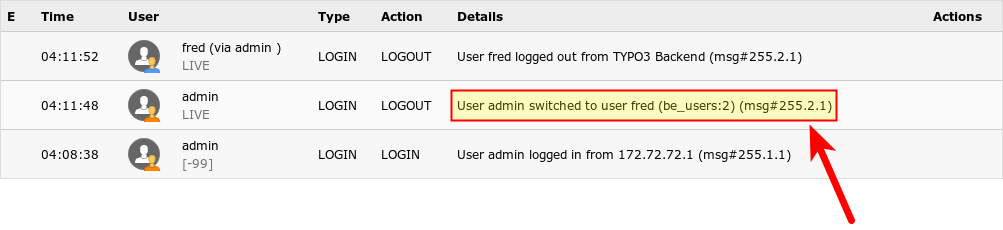
\includegraphics[width=0.90\linewidth]{InDepthChanges/78432-SwitchUserActionLogMessage.png}
	\end{figure}

\end{frame}

% ------------------------------------------------------------------------------
% Feature | 83734 | Add support for current page in configcache
% Breaking | 88564 | PageTSconfig setting TSFE.constants removed
% Breaking | 88657 | Popup configuration in FormEngine dropped

\begin{frame}[fragile]
	\frametitle{Changements en profondeur}
	\framesubtitle{Changements TypoScript (1)}

	\begin{itemize}
		\item La propriété TypoScript \texttt{config.cache} supporte le mot-clé
			«~\texttt{current}~» référençant la page courante. Par exemple~: \newline
			\smaller\texttt{config.cache.all = fe\_users:current}\normalsize

		\item L'option de configuration Page/User TSconfig \texttt{TSFE.constants} est retirée.

			\begin{itemize}\smaller
				\item[\ding{228}] Incluez les conditions TypoScript dans la configuration et les constantes,
				et utilisez une configuration adéquate dans le fichier \texttt{ext\_localconf.php}.
			\end{itemize}

		\item Ces deux options de configuration de la taille des fenêtres popup sont retirées~:

			\begin{itemize}
				\item \texttt{options.popupWindowSize}
				\item \texttt{options.rte.popupWindowSize}
			\end{itemize}

	\end{itemize}

\end{frame}

% ------------------------------------------------------------------------------
% Breaking | 88640 | Database field sys_template.nextLevel and TypoScript sublevel inheritance removed
% Task | 88755 | Remove POST option from typolink.addQueryString

\begin{frame}[fragile]
	\frametitle{Changements en profondeur}
	\framesubtitle{Changements TypoScript (2)}

	\begin{itemize}
		\item Le champ de base de données \texttt{nextLevel} de la table
			\texttt{sys\_template} est retiré.

			\begin{itemize}\smaller
				\item[\ding{228}] Remplacez l'enregistrement (l'identifiant est enregistré dans le champ
					\texttt{nextLevel}) par une condition TypoScript pour les sous-pages.
					Par exemple~: \texttt{[tree.level > 1]}
			\end{itemize}\normalsize

		\item Les valeurs suivantes \textbf{ne sont plus permises}~:

			\begin{itemize}\smaller
				\item \texttt{typolink.addQueryString.method = POST}
				\item \texttt{typolink.addQueryString.method = GET,POST}
				\item \texttt{typolink.addQueryString.method = POST,GET}
			\end{itemize}\normalsize

			\begin{itemize}\smaller
				\item[\ding{228}] Changez les affectations TypoScript, Fluid et PHP par \texttt{GET}.
			\end{itemize}\normalsize

	\end{itemize}

\end{frame}

% ------------------------------------------------------------------------------
% 87499 | Drop extensions "taskcenter" and "sys_action" from core

\begin{frame}[fragile]
	\frametitle{Changements en profondeur}
	\framesubtitle{Centre de tâches et \texttt{EXT:sys\_action}}

	\begin{itemize}

		\item Les extensions système \texttt{EXT:taskcenter} et \texttt{EXT:sys\_action}
			ne font plus parties du cœur.

		\item Elles sont disponibles en extensions indépendantes depuis le
			\href{https://extensions.typo3.org/}{TER}
			et sur \href{https://github.com/FriendsOfTYPO3}{GitHub}.

		\item Le tableau de bord remplace les centre de tâches et \texttt{EXT:sys\_action}.

	\end{itemize}

\end{frame}

% ------------------------------------------------------------------------------
% Feature | 89227 | Ask for email address while installing TYPO3

\begin{frame}[fragile]
	\frametitle{Changements en profondeur}
	\framesubtitle{Adresse email administrateur}

	\begin{columns}[T]
		\begin{column}{.04\textwidth}
		\end{column}
		\begin{column}{.38\textwidth}

			La saisie d'une adresse email fait partie de la procédure d'installation.
			Cette adresse est utilisée pour le premier administrateur du backend.

			\vspace{0.2cm}

			L'option existe aussi dans l'action \textbf{Create Administrative User} du
			module de maintenance de l'outil d'installation.

		\end{column}
		\begin{column}{.58\textwidth}
			\vspace{-0.3cm}
			\begin{figure}
				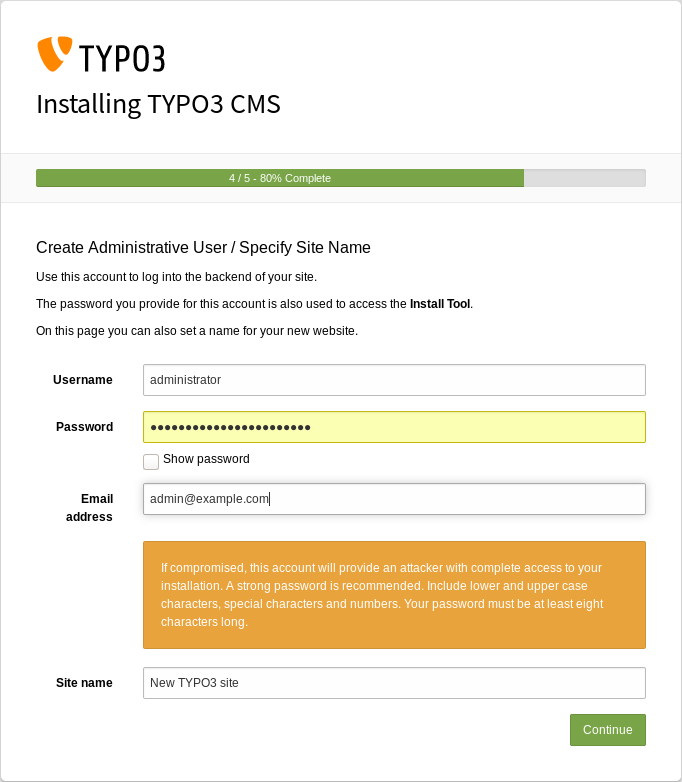
\includegraphics[width=0.70\linewidth]{InDepthChanges/89227-EmailAddressDuringInstallation.png}
			\end{figure}
		\end{column}
	\end{columns}

\end{frame}

% ------------------------------------------------------------------------------
% Breaking | 87583 | Remove obsolete APC Cache Backend implementation
% Breaking | 87558 | Consolidate extbase caches

\begin{frame}[fragile]
	\frametitle{Changements en profondeur}
	\framesubtitle{Caches}

	% decrease font size for code listing
	\lstset{basicstyle=\tiny\ttfamily}

	\begin{itemize}
		\item Le framework de cache ne supporte plus \texttt{ApcBackend}

			\begin{itemize}\smaller
				\item[\ding{228}] Utilisez \textbf{APCu} en remplacement - notez le «~u~».
			\end{itemize}

\begin{lstlisting}
ANCIEN :
\$GLOBALS['TYPO3_CONF_VARS']['SYS']['caching']['cacheConfigurations']['rootline']['backend'] =
\TYPO3\CMS\Core\Cache\Backend\ApcBackend::class;

NOUVEAU :
\$GLOBALS['TYPO3_CONF_VARS']['SYS']['caching']['cacheConfigurations']['rootline']['backend'] = \TYPO3\CMS\Core\Cache\Backend\ApcuBackend::class;
	\end{lstlisting}

		\item Les caches Extbase \texttt{extbase\_reflection} et \texttt{extbase\_datamapfactory\_datamap}
			ont été consolidés et sont disponibles sous un seul cache nommé «~\texttt{extbase}~».

	\end{itemize}

\end{frame}

% ------------------------------------------------------------------------------
% Feature | 89229 | Cache Preset for Settings in Maintenance Area

\begin{frame}[fragile]
	\frametitle{Changements en profondeur}
	\framesubtitle{Type de stockage des caches (1)}

	\begin{itemize}

		\item TYPO3 fournit un système de cache flexible avec une configuration
			par défaut idéale dans la plupart des cas.
		\item Le type de stockage est configurable pour affiner les caches et
			augmenter les performances en fonction de l'environnement.

		\begin{itemize}
			\item Choisir le stockage en \textbf{base de données} pour un environnement classique
				ou si, par exemple, un système de fichiers réseau (NFS) est utilisé.
			\item Choisir le stockage sur le \textbf{système de fichiers} si, par exemple,
				une base de données distribuée est utilisée.
			\item Choisir des \textbf{paramètres de cache sur mesure} afin de configurer les types de stockage
				de façon indépendante.
		\end{itemize}

		\item Dans le cas d'installations plus complexes, des caches mémoire comme
			\href{https://redis.io/}{Redis}
			ou
			\href{https://memcached.org/}{Memcached} sont à étudier.

	\end{itemize}

\end{frame}

% ------------------------------------------------------------------------------
% Feature | 89229 | Cache Preset for Settings in Maintenance Area

\begin{frame}[fragile]
	\frametitle{Changements en profondeur}
	\framesubtitle{Type de stockage des caches (2)}

	Outils d'administration \ding{223}\hspace{0.1cm}Réglages \ding{223}\hspace{0.1cm}Configuration Presets \ding{223}\hspace{0.1cm}Cache Settings~:

	\begin{figure}
		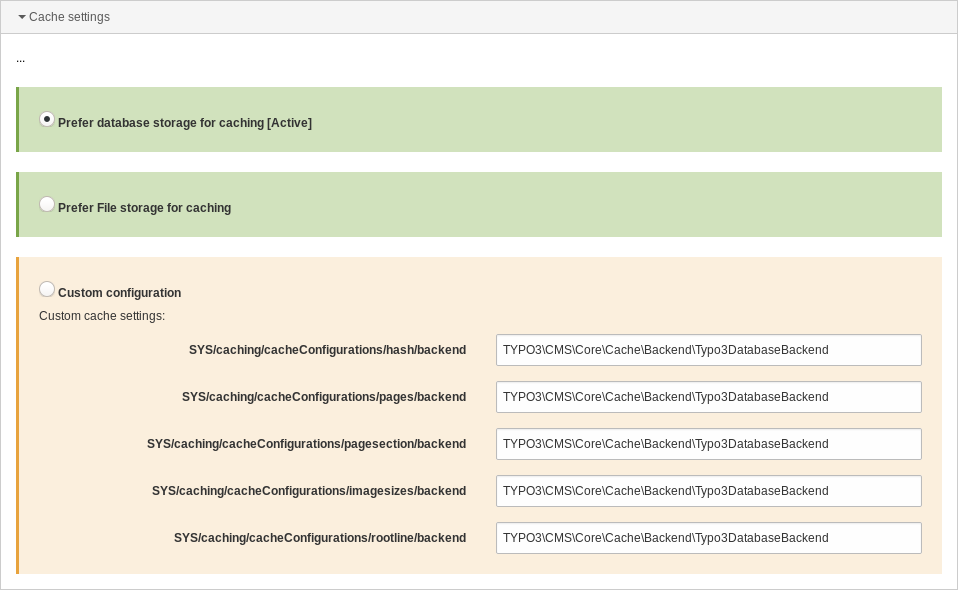
\includegraphics[width=0.70\linewidth]{InDepthChanges/89229a-CachePresetForSettingsInMaintenanceArea.png}
	\end{figure}

\end{frame}

% ------------------------------------------------------------------------------
% Feature | 89054 | Provide core cache frontends via dependency injection

\begin{frame}[fragile]
	\frametitle{Changements en profondeur}
	\framesubtitle{Injection du cache par dépendance (1)}

	% decrease font size for code listing
	\lstset{basicstyle=\tiny\ttfamily}

	\begin{itemize}
		\item Les développeurs d'extension sont encouragés à injecter les caches directement plutôt
			que d'utiliser CacheManager.
		\item Les changements requis sont à effectuer comme suit.

		\item \textbf{Précédemment~:}
\begin{lstlisting}
class MyClass
{
  /**
   * @var TYPO3\CMS\Core\Cache\Frontend\FrontendInterface
   */
  private \$cache;

  public function __construct()
  {
      \$cacheManager = GeneralUtility::makeInstance(CacheManager::class);
      \$this->cache = \$cacheManager->getCache('my_cache');
  }
}
\end{lstlisting}

	\end{itemize}

\end{frame}

% ------------------------------------------------------------------------------
% Feature | 89054 | Provide core cache frontends via dependency injection

\begin{frame}[fragile]
	\frametitle{Changements en profondeur}
	\framesubtitle{Injection du cache par dépendance (2)}

	% decrease font size for code listing
	\lstset{basicstyle=\tiny\ttfamily}

	\begin{itemize}
		\item Dans \textbf{TYPO3 v10 LTS}, la classe doit être comme ci-dessous~:
\begin{lstlisting}
class MyClass
{
  /**
   * @var TYPO3\CMS\Core\Cache\Frontend\FrontendInterface
   */
  private \$cache;

  public function __construct(FrontendInterface \$cache)
  {
    \$this->cache = \$cache;
  }
}
\end{lstlisting}

	\end{itemize}

\end{frame}

% ------------------------------------------------------------------------------
% Feature | 89054 | Provide core cache frontends via dependency injection

\begin{frame}[fragile]
	\frametitle{Changements en profondeur}
	\framesubtitle{Injection du cache par dépendance (3)}

	% decrease font size for code listing
	\lstset{basicstyle=\tiny\ttfamily}

	\begin{itemize}
		\item \ldots et la configuration de service suivante est requise~:
\begin{lstlisting}
services:
  cache.my_cache:
    class: TYPO3\CMS\Core\Cache\Frontend\FrontendInterface
    factory: ['@TYPO3\CMS\Core\Cache\CacheManager', 'getCache']
    arguments: ['my_cache']

  MyClass:
    arguments:
      \$cache: '@cache.my_cache'
\end{lstlisting}

	\end{itemize}

\end{frame}

% ------------------------------------------------------------------------------
% Deprecation | 88366 | Default caching framework cache names changed

\begin{frame}[fragile]
	\frametitle{Changements en profondeur}
	\framesubtitle{Framework de cache}

	% decrease font size for code listing
	\lstset{basicstyle=\tiny\ttfamily}

	\begin{itemize}
		\item Les caches suivants sont renommés~:

			\begin{itemize}\smaller
				\item \texttt{cache\_core} \textrightarrow\hspace{0.1cm}\texttt{core}
				\item \texttt{cache\_hash} \textrightarrow\hspace{0.1cm}\texttt{hash}
				\item \texttt{cache\_pages} \textrightarrow\hspace{0.1cm}\texttt{pages}
				\item \texttt{cache\_pagesection} \textrightarrow\hspace{0.1cm}\texttt{pagesection}
				\item \texttt{cache\_runtime} \textrightarrow\hspace{0.1cm}\texttt{runtime}
				\item \texttt{cache\_rootline} \textrightarrow\hspace{0.1cm}\texttt{rootline}
				\item \texttt{cache\_imagesizes} \textrightarrow\hspace{0.1cm}\texttt{imagesizes}
			\end{itemize}\normalsize

		\item Nouvelle méthode d'accès aux caches~:

\begin{lstlisting}
AVANT :
\$cacheManager->getCache('cache_core').

MAINTENANT :
\$cacheManager->getCache('core')
\end{lstlisting}

		\item Le préfixe \texttt{cf\_} est retiré des tables de base de données.
	\end{itemize}

\end{frame}

% ------------------------------------------------------------------------------
% Feature | 89090 | Reports for conflicting redirects

\begin{frame}[fragile]
	\frametitle{Changements en profondeur}
	\framesubtitle{Conflits de redirection (1)}

	\begin{itemize}
		\item Une commande Symfony est introduite pour la détection des redirections
			en conflit avec les URLs de page.
		\item Exécuter la commande CLI~:\newline
			\smaller
				(le paramètre optionnel \texttt{-}\texttt{-site} limite la vérification à un site spécifique)
			\normalsize
	\end{itemize}

	\begin{figure}
		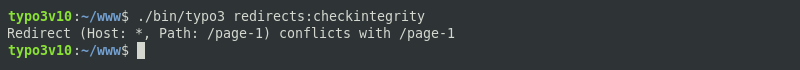
\includegraphics[width=0.90\linewidth]{InDepthChanges/89090a-ReportsForConflictingRedirects.png}
	\end{figure}

	\begin{itemize}
		\item Cette commande est aussi disponible dans le planificateur~:
	\end{itemize}

	\begin{figure}
		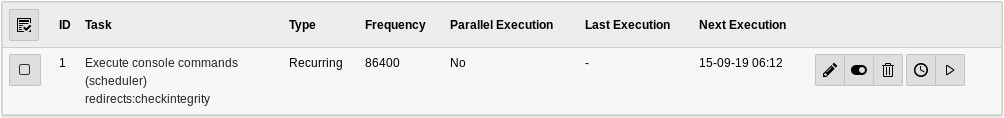
\includegraphics[width=0.90\linewidth]{InDepthChanges/89090b-ReportsForConflictingRedirects.png}
	\end{figure}

\end{frame}

% ------------------------------------------------------------------------------
% Feature | 89090 | Reports for conflicting redirects

\begin{frame}[fragile]
	\frametitle{Changements en profondeur}
	\framesubtitle{Conflits de redirection (2)}

	\begin{itemize}
		\item La liste des conflits de redirections est aussi disponible dans le module Rapports~:
	\end{itemize}

	\begin{figure}
		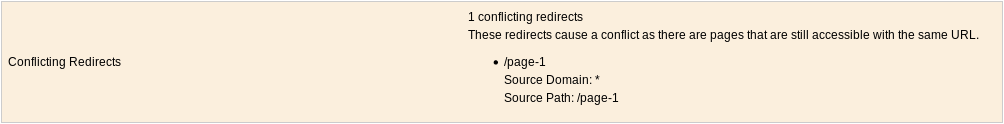
\includegraphics[width=0.90\linewidth]{InDepthChanges/89090c-ReportsForConflictingRedirects.png}
	\end{figure}

	\begin{itemize}
		\item
			\small\textbf{Note~:}
				La commande doit être exécutée de nouveau pour réinitialiser la liste.
				Résoudre les problèmes (i.e. retirer la redirection) ne vide pas la liste.
			\normalsize
	\end{itemize}

\end{frame}

% ------------------------------------------------------------------------------
% Feature | 89010 | Introduce Site Configuration for Distribution Packages

\begin{frame}[fragile]
	\frametitle{Changements en profondeur}
	\framesubtitle{Distributions}

	% decrease font size for code listing
	\lstset{basicstyle=\tiny\ttfamily}

	\begin{itemize}
		\item Les distributions peuvent fournir leurs fichiers de configuration de site.

		\item Créer un dossier / fichier dans l'archive de la distribution comme suit~:\newline
			\texttt{Initialisation/Site/<siteIdentifier>/config.yaml}

		\item Comme les ressources, qui sont déplacées dans le dossier \texttt{fileadmin/},\newline
			les configurations de site sont déplacées dans le dossier \texttt{config/}.

		\item Si le répertoire cible existe déjà, aucun de changement de configuration n'est effectué.
	\end{itemize}

\end{frame}

% ------------------------------------------------------------------------------
% Feature | 88318 | Display Application Context in CLI

\begin{frame}[fragile]
	\frametitle{Changements en profondeur}
	\framesubtitle{Contexte d'application en CLI}

	\begin{itemize}
		\item Le contexte d'application actuel apparaît à côté de la version de
			TYPO3 dans les requêtes CLI~:
	\end{itemize}

	\begin{figure}
		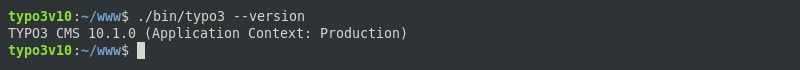
\includegraphics[width=0.90\linewidth]{InDepthChanges/88318-DisplayApplicationContextInCli.png}
	\end{figure}

\end{frame}

% ------------------------------------------------------------------------------
% Feature | 87525 | Add api=1 option in VimeoRenderer

\begin{frame}[fragile]
	\frametitle{Changements en profondeur}
	\framesubtitle{Rendu des vidéos Vimeo}

	% decrease font size for code listing
	\lstset{basicstyle=\smaller\ttfamily}

	\begin{itemize}
		\item Le paramètre \texttt{api=1} des URLs Vimeo autorise les interactions
			avec l'API du lecteur (par exemple~: ajout de boutons de contrôle vidéo).
		\item Les intégrateurs peuvent déclarer ce paramètre de deux façons~:

		\begin{itemize}
			\item En TypoScript~:

\begin{lstlisting}
lib.contentElement.settings.media.additionalConfig.api = 1
\end{lstlisting}

			\item Dans Fluid en utilisant le ViewHelper Media~:
\begin{lstlisting}
<f:media
  file="{file}"
  alt="{file.properties.alternative}"
  title="{file.properties.title}"
  additionalConfig="{api: 1}"
/>
\end{lstlisting}

		\end{itemize}
	\end{itemize}

\end{frame}

% ------------------------------------------------------------------------------
% Feature | 86670 | Make default action in DragUploader adjustable

\begin{frame}[fragile]
	\frametitle{Changements en profondeur}
	\framesubtitle{Chargement de fichiers}

	% decrease font size for code listing
	\lstset{basicstyle=\smaller\ttfamily}

	\begin{itemize}
		\item Il est possible de configurer l'action par défaut lorsqu'on charge des fichiers
			à l'aide du glisser-déplacer du module de liste des fichiers.
		\item User TSConfig~:

\begin{lstlisting}
# Set default to replace:
options.file_list.uploader.defaultAction = replace

# Set default to rename:
options.file_list.uploader.defaultAction = rename

# Set default to cancel:
options.file_list.uploader.defaultAction = cancel
\end{lstlisting}

	\end{itemize}

\end{frame}

% ------------------------------------------------------------------------------
% Feature | 84250 | Separately enable / disable "Add media by URL" and "Select & upload files"

\begin{frame}[fragile]
	\frametitle{Changements en profondeur}
	\framesubtitle{Boutons des éléments média}

	% decrease font size for code listing
	\lstset{basicstyle=\tiny\ttfamily}

	\begin{itemize}
		\item Les boutons \textbf{«~Ajouter un média à partir d’une URL~»} et
			\textbf{«~Sélectionner et transférer des fichiers~»} sont activables
			/ désactivables indépendamment.
	\end{itemize}

	\begin{figure}
		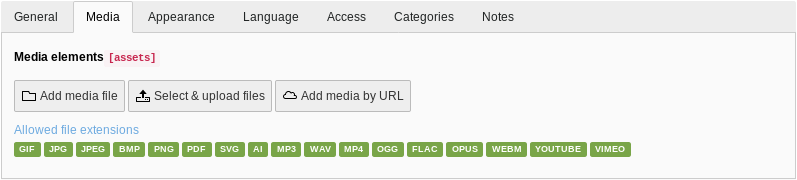
\includegraphics[width=0.75\linewidth]{InDepthChanges/84250-EnableDisableMediaButtons.png}
	\end{figure}

	\begin{itemize}
		\item L'exemple ci-dessous montre comment cacher les deux boutons~:
\begin{lstlisting}
\$GLOBALS['TCA']['pages']['columns']['media']['config']['appearance'] = [
  'fileUploadAllowed' => false,
  'fileByUrlAllowed' => false,
];
\end{lstlisting}

	\end{itemize}

\end{frame}

% ------------------------------------------------------------------------------
% Feature | 88441 | Show configuration of USER_INT objects in adminpanel

\begin{frame}[fragile]
	\frametitle{Changements en profondeur}
	\framesubtitle{Panneau d'administrateur}

	\begin{itemize}
		\item Le panneau d'administrateur inclus un panneau \textbf{USER\_INT} sous le module Info.
	\end{itemize}

	\begin{figure}
		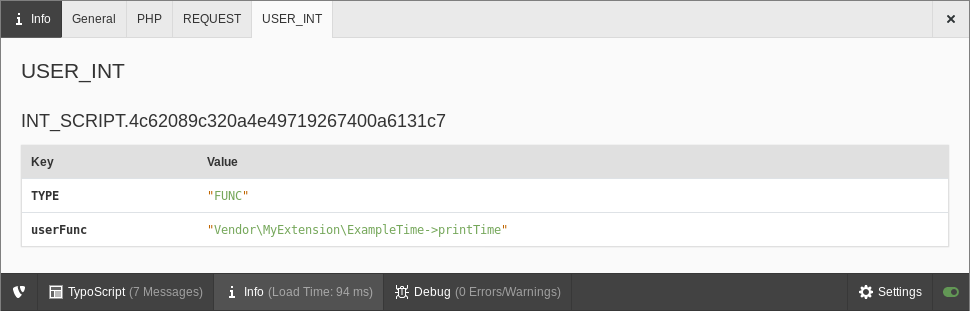
\includegraphics[width=0.90\linewidth]{InDepthChanges/88441-ShowUserIntObjectsInAdminPanel.png}
	\end{figure}

\end{frame}

% ------------------------------------------------------------------------------
% Feature | 89142 | Create site configuration if page is created on root level

\begin{frame}[fragile]
	\frametitle{Changements en profondeur}
	\framesubtitle{Configuration de Site (1)}

	\begin{itemize}
		\item À la création d'une nouvelle page au niveau racine, une configuration
			de site standard est automatiquement générée.
		\item On peut donc créer un site TYPO3 rapidement.
		\item La configuration contient~:

			\begin{itemize}
				\item Un identifiant prédéfinit (i.e. \texttt{site-42-a1d0c6e83f})
				\item Un point d'entrée (i.e. \texttt{https://example.com/site-42})
				\item Une langue par défaut (i.e. \texttt{English})
			\end{itemize}

	\end{itemize}

\end{frame}

% ------------------------------------------------------------------------------
% Feature | 85592 | Add site title configuration to sites module

\begin{frame}[fragile]
	\frametitle{Changements en profondeur}
	\framesubtitle{Configuration de site (2)}

	\begin{itemize}

		\item Le titre du site se configure dans
			\textbf{Gestionnaire de site} $\rightarrow$ \textbf{Sites}.
		\item Les intégrateurs peuvent spécifier un titre de site différent pour chaque langues.
		\item Le champ de l'enregistrement gabarit est obsolète et marqué \textbf{déprécié}.
		\item Le champ \texttt{sys\_template.sitetitle} (base et TCA) sera retiré de TYPO3 v11.
		\item Le titre du site est utilisé pour le titre de page et pour les intégrations futures de
			\texttt{schema.org}.
	\end{itemize}

\end{frame}

% ------------------------------------------------------------------------------
% Feature | 89398 | Support for environment variables in imports in site configurations

\begin{frame}[fragile]
	\frametitle{Changements en profondeur}
	\framesubtitle{Configuration de site (3)}

	% decrease font size for code listing
	\lstset{basicstyle=\tiny\ttfamily}

	\begin{itemize}

		\item Les variables d'environnement sont utilisables dans les importations des fichiers YAML de
			configuration de site~:
\begin{lstlisting}
imports:
  -
    resource: 'Env_%env("foo")%.yaml'
\end{lstlisting}

	\end{itemize}

\end{frame}

% ------------------------------------------------------------------------------
% Feature | 88102 | Frontend Login Form Via Fluid And Extbase

\begin{frame}[fragile]
	\frametitle{Changements en profondeur}
	\framesubtitle{Authentification frontend (1)}

	\begin{itemize}

		\item TYPO3 v10 LTS inclus une version basée sur Extbase de l'authentification frontend.
		\item La solution présentes les avantages~:

			\begin{itemize}
				\item Aisance de modification du gabarit.
				\item Envoie d'email de récupération de mot de passe au format HTML\@.
				\item Ajustement et modification des validateurs pour forcer les restrictions sur les mots de passe.
			\end{itemize}

		\item Le plugin est directement disponible dans les nouvelles installations.
		\item Les instances TYPO3 existantes continuerons d'utiliser les anciens gabarits.
		\item Les intégrateurs peuvent basculer entre l'ancien et le nouveau plugin dans la configuration des fonctionnalités.

	\end{itemize}

\end{frame}

% ------------------------------------------------------------------------------
% Feature | 88110 | Felogin extbase password recovery

\begin{frame}[fragile]
	\frametitle{Changements en profondeur}
	\framesubtitle{Authentification frontend (2)}

	\begin{itemize}

		\item Le formulaire de récupération de mot de passe est intégré au plugin Extbase.
		\item Les utilisateurs peuvent demander un changement de mot de passe. Ils recevront
			un email avec un lien les redirigeant vers le formulaire.
		\item Règles de validation de mots de passe par défaut~:

			\begin{itemize}
				\item \texttt{NotEmptyValidator} - les mots de passe ne sont pas vides.
				\item \texttt{StringLengthValidator} - les mots de passe ont une longueur minimale.
			\end{itemize}

	\end{itemize}

\end{frame}

% ------------------------------------------------------------------------------
% Feature | 88110 | Felogin extbase password recovery

\begin{frame}[fragile]
	\frametitle{Changements en profondeur}
	\framesubtitle{Authentification frontend (3)}

	% decrease font size for code listing
	\lstset{basicstyle=\tiny\ttfamily}

	\begin{itemize}
		\item Ces règles de validation sont personnalisables.
		\item Par exemple~:
\begin{lstlisting}
plugin.tx_felogin_login {
  settings {
    passwordValidators {
      10 = TYPO3\CMS\Extbase\Validation\Validator\AlphanumericValidator
      20 {
        className = TYPO3\CMS\Extbase\Validation\Validator\StringLengthValidator
        options {
          minimum = 12
          maximum = 32
        }
      }
      30 = \Vendor\MyExtension\Validation\Validator\MyCustomPasswordPolicyValidator
    }
  }
}
\end{lstlisting}

	\end{itemize}

\end{frame}

% ------------------------------------------------------------------------------
% Feature | 89171 | Added possibility to have multiple sitemaps

\begin{frame}[fragile]
	\frametitle{Changements en profondeur}
	\framesubtitle{Sitemap multiples}

	% decrease font size for code listing
	\lstset{basicstyle=\tiny\ttfamily}

	\begin{itemize}

		\item Il est possible de définir de multiples sitemaps.
		\item Syntaxe~:
\begin{lstlisting}
plugin.tx_seo {
  config {
    <sitemapType> {
      sitemaps {
        <unique key> {
          provider = TYPO3\CMS\Seo\XmlSitemap\RecordsXmlSitemapDataProvider
          config {
            ...
          }
        }
      }
    }
  }
}
\end{lstlisting}

	\end{itemize}

\end{frame}

% ------------------------------------------------------------------------------
% Feature | 86759 | Support nomodule attribute for JavaScript includes

\begin{frame}[fragile]
	\frametitle{Changements en profondeur}
	\framesubtitle{Attribut HTML5 \texttt{nomodule}}

	% decrease font size for code listing
	\lstset{basicstyle=\tiny\ttfamily}

	\begin{itemize}
		\item L'attribut HTML5 \texttt{nomodule} est supporté lors de l'inclusion de fichiers JavaScript en TypoScript.
\begin{lstlisting}
page.includeJSFooter.file = path/to/classic-file.js
page.includeJSFooter.file.nomodule = 1
\end{lstlisting}

		\item L'attribut empêche l'exécution du script lorsque le navigateur supporte les scripts modulaires.

		\item En savoir plus sur le standard dans la
			\href{https://html.spec.whatwg.org/multipage/scripting.html#attr-script-nomodule}{spécification}
			et sur le concept de
			\href{https://hacks.mozilla.org/2015/08/es6-in-depth-modules/}{modules}.

	\end{itemize}

% <script type="module" src="path/to/file.js"></script>
% <script nomodule src="path/to/file/classic-file.js"></script>

\end{frame}

% ------------------------------------------------------------------------------
% Feature | 86918 | Add additional configuration for external link types in Linkvalidator

\begin{frame}[fragile]
	\frametitle{Changements en profondeur}
	\framesubtitle{Validateur de liens (1)}

	% decrease font size for code listing
	\lstset{basicstyle=\tiny\ttfamily}

	\begin{itemize}
		\item Le validateur de lien supporte des configurations supplémentaires pour les liens externes.
		\item Les valeurs pour \texttt{httpAgentUrl} et \texttt{httpAgentEmail} devraient être fournies.
		\item Les options \texttt{headers}, \texttt{method} et \texttt{range} sont pour l'usage avancé.
\begin{lstlisting}
mod.linkvalidator {
  linktypesConfig {
    external {
      httpAgentName = \ldots
      httpAgentUrl = \ldots
      httpAgentEmail = \ldots
      headers {
      }
      method = HEAD
      range = 0-4048
    }
  }
}
\end{lstlisting}

	\end{itemize}

\end{frame}

% ------------------------------------------------------------------------------
% Feature | 84990 | Add event for checking external links in RTE

\begin{frame}[fragile]
	\frametitle{Changements en profondeur}
	\framesubtitle{Validateur de liens (2)}

	\begin{itemize}
		\item Le validateur de lien marque les liens \textbf{externe} cassés dans le RTE\@.
		\item La fonction n'est disponible que pour les liens internes.
		\item Il est recommandé de mettre en place la tâche planifiée du validateur de lien pour
			chercher régulièrement les liens cassés.
	\end{itemize}

\end{frame}

% ------------------------------------------------------------------------------



% ------------------------------------------------------------------------------
% Important | 89992 | Use New TranslationServer
% Feature | 89526 | FeatureFlag: betaTranslationServer

\begin{frame}[fragile]
	\frametitle{Changements en profondeur}
	\framesubtitle{Plateforme de gestion des traductions}

	\begin{itemize}
		\item La solution SaaS \href{https://crowdin.com/}{Crowdin} est maintenant la
			plateforme de gestion des traductions pour TYPO3.
		\item Nous encourageons tous le monde à participer et améliorer la traduction.
		\item Crowdin est utilisé pour traduire les libellés de langue du noyau de TYPO3
			ainsi que ceux des extensions TYPO3.
		\item En savoir plus sur l'initiative dans
			\href{https://typo3.org/community/teams/typo3-development/initiatives/localization-with-crowdin/}{cet article (en)}
			et dans la
			\href{https://docs.typo3.org/m/typo3/reference-coreapi/master/en-us/ApiOverview/Internationalization/TranslationServer/Crowdin.html}{documentation TYPO3 (en)}.
	\end{itemize}

	\begin{figure}
		
\includegraphics[width=0.40\linewidth]{InDepthChanges/crowdin-logo.png}
	\end{figure}

\end{frame}

% ------------------------------------------------------------------------------
% Feature | 90266 | Fluid-based templated emails

\begin{frame}[fragile]
	\frametitle{Changements en profondeur}
	\framesubtitle{Emails HTML basés sur Fluid (1)}

	% decrease font size for code listing
	\lstset{basicstyle=\smaller\ttfamily}

	\begin{itemize}
		\item Les contenus des emails HTML et texte brute sont basés sur des templates.
		\item Ils sont générés à l'aide du moteur de rendu Fluid.
		\item La personnalisation s'effectue en surchargeant les chemins vers les fichiers~:
\begin{lstlisting}
\$GLOBALS['TYPO3_CONF_VARS']['MAIL']['templateRootPaths'][700] =
  'EXT:my_site_extension/Resources/Private/Templates/Email';

\$GLOBALS['TYPO3_CONF_VARS']['MAIL']['layoutRootPaths'][700] =
  'EXT:my_site_extension/Resources/Private/Layouts';
\end{lstlisting}

	\end{itemize}

\end{frame}

% ------------------------------------------------------------------------------
% Feature | 90266 | Fluid-based templated emails

\begin{frame}[fragile]
	\frametitle{Changements en profondeur}
	\framesubtitle{Emails HTML basés sur Fluid (2)}

	\begin{itemize}
		\item Par exemple, les composants suivants utilisent les templates Fluid~:

			\begin{itemize}
				\item Message de test de l'outil d'installation (voir l'exemple sur la prochaine diapositive).
				\item Messages de notification des espaces de travail lors du changement d'étape.
				\item Message de notification de connexion d'un utilisateur backend.
			\end{itemize}

	\end{itemize}

\end{frame}

% ------------------------------------------------------------------------------
% Feature | 90266 | Fluid-based templated emails

\begin{frame}[fragile]
	\frametitle{Changements en profondeur}
	\framesubtitle{Emails HTML basés sur Fluid (3)}

	Message de test envoyé depuis l'outil d'installation~:

	\begin{figure}
		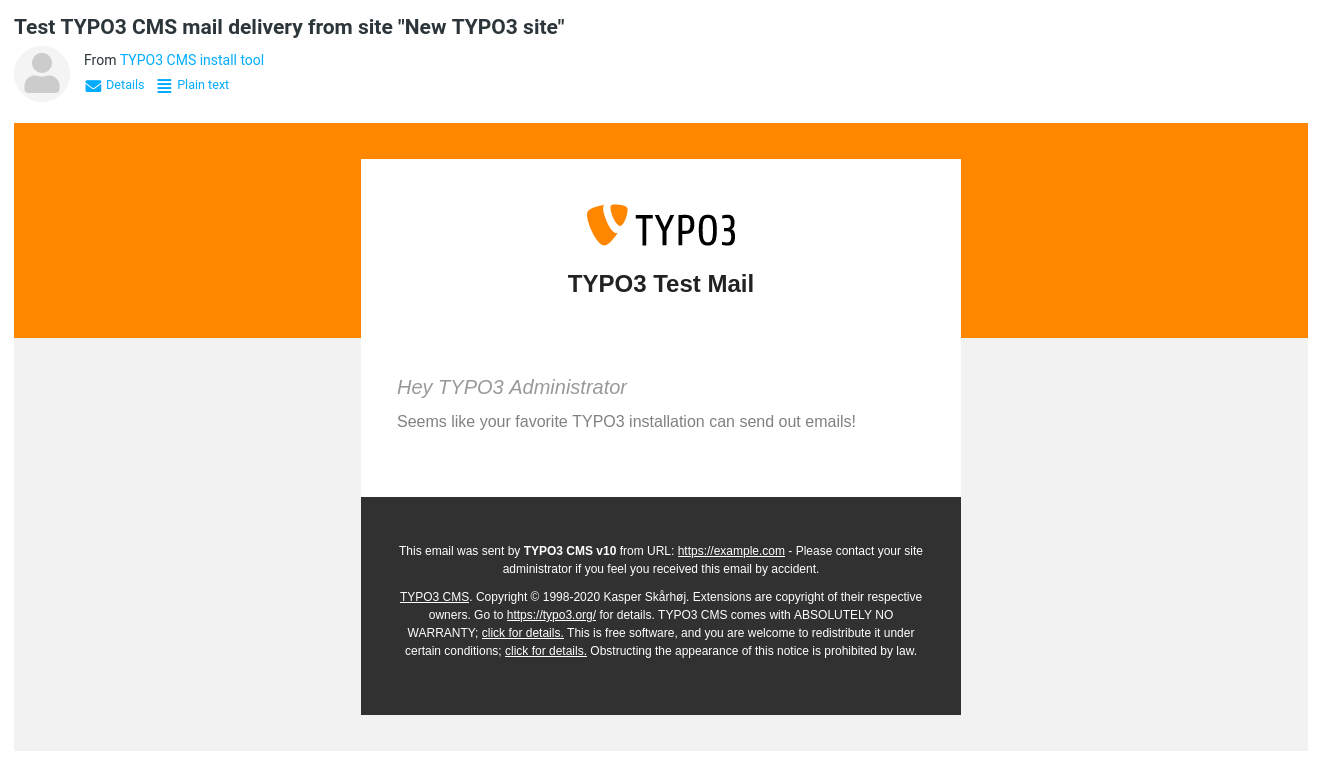
\includegraphics[width=0.8\linewidth]{InDepthChanges/90266-FluidBasedTemplatedEmails.png}
	\end{figure}

\end{frame}

% ------------------------------------------------------------------------------
% Feature | 88962 | Re-implement old PIDupinRootline TypoScript condition

\begin{frame}[fragile]
	\frametitle{Changements en profondeur}
	\framesubtitle{TypoScript}

	% decrease font size for code listing
	\lstset{basicstyle=\smaller\ttfamily}

	\begin{itemize}
		\item L'ancienne condition \texttt{PIDupinRootline} est réimplémenté
			en TypoScript dans le langage d'expression de Symfony.
		\item Ancienne syntaxe de la condition TypoScript~:

\vspace{-0.4cm}
\begin{lstlisting}
[PIDupinRootline = 30]
  page.10.value = I'm on any subpage of page with UID 30.
[END]
\end{lstlisting}

		\item Nouvelle syntaxe de la condition TypoScript~:
\begin{lstlisting}
[30 in tree.rootLineParentIds]
  page.10.value = I'm on any subpage of page with UID 30.
[END]
\end{lstlisting}

	\end{itemize}

\end{frame}

% ------------------------------------------------------------------------------
% Feature | 90426 | Browser-native lazy loading for images

\begin{frame}[fragile]
	\frametitle{Changements en profondeur}
	\framesubtitle{Chargement différé des images}

	% decrease font size for code listing
	\lstset{basicstyle=\smaller\ttfamily}

	\begin{itemize}
		\item L'attribut HTML \texttt{loading} est disponible pour les balises \texttt{<img>}.
		\item Les navigateurs supportant cette fonctionnalité ne chargeront pas ces images
			avant qu'elles soient visibles.
		\item Le comportement est modifiable avec la constante TypoScript suivante~:

\vspace{-0.4cm}
\begin{lstlisting}
styles.content.image.lazyLoading = lazy
\end{lstlisting}

		\item Les valeurs valides sont~: \texttt{lazy} (default), \texttt{eager}, et \texttt{auto}.
		\item Le ViewHelper Fluid \textit{Image} supporte aussi cet attribut~:
\begin{lstlisting}
<f:image src="{fileObject}" treatIdAsReference="true"
  loading="lazy" />
\end{lstlisting}

	\end{itemize}

\end{frame}

% ------------------------------------------------------------------------------
% Important | 89869 | Change lockIP default to disabled for both frontend and backend

\begin{frame}[fragile]
	\frametitle{Changements en profondeur}
	\framesubtitle{Valeurs par défaut pour \texttt{lockIP}/\texttt{lockIPv6}}

	% decrease font size for code listing
	\lstset{basicstyle=\smaller\ttfamily}

	\begin{itemize}
		\item Les valeurs par défaut pour les options \texttt{lockIP} ont changées.
		\item Ces quatre variables système suivantes sont \textbf{désactivées} par défaut~:

			\begin{itemize}
				\item \texttt{[FE]['lockIP']}
				\item \texttt{[FE]['lockIPv6']}
				\item \texttt{[BE]['lockIP']}
				\item \texttt{[BE]['lockIPv6']}
			\end{itemize}

		\item Les anciennes valeur par défaut (\texttt{4} pour le backend et \texttt{2} pour le frontend)
			posaient des problèmes pour les clients supportant IPv4 et IPv6.

	\end{itemize}

\end{frame}

% ------------------------------------------------------------------------------
% Feature | 88147 | Add possibility to configure the path to sitemap xslFile

\begin{frame}[fragile]
	\frametitle{Changements en profondeur}
	\framesubtitle{SEO~: \texttt{Sitemap.xsl}}

	% decrease font size for code listing
	\lstset{basicstyle=\tiny\ttfamily}

	\begin{itemize}
		\item Le chemin par défaut du fichier \texttt{Sitemap.xsl} de l'extension
			système \texttt{EXT:seo} est modifiable~:
\begin{lstlisting}
# Globally for all sitemaps:
plugin.tx_seo.config.xslFile = EXT:myext/Resources/Public/CSS/mySite.xsl

# For all sitemaps of a specific type:
plugin.tx_seo.config.<sitemapType>.sitemaps.xslFile = EXT:myext/Resources/Public/CSS/mySite.xsl

# For a specific sitemap:
plugin.tx_seo.config.<sitemapType>.sitemaps.<sitemap>.config.xslFile =
  EXT:myext/Resources/Public/CSS/mySite.xsl
\end{lstlisting}

		\item Le chemin par défaut est~:\newline
			\smaller
				\texttt{EXT:seo/Resources/Public/CSS/Sitemap.xsl}
			\normalsize

	\end{itemize}

\end{frame}

% ------------------------------------------------------------------------------
% Feature | 82062 | Progress for Reference Index update on CLI

\begin{frame}[fragile]
	\frametitle{Changements en profondeur}
	\framesubtitle{Index des références}

	% decrease font size for code listing
	\lstset{basicstyle=\tiny\ttfamily}

	\begin{itemize}
		\item Pendant la mise à jour de l'index des références, des barres de progression sont
			affichées pour chaque tables de la base.
	\end{itemize}

	\begin{figure}
		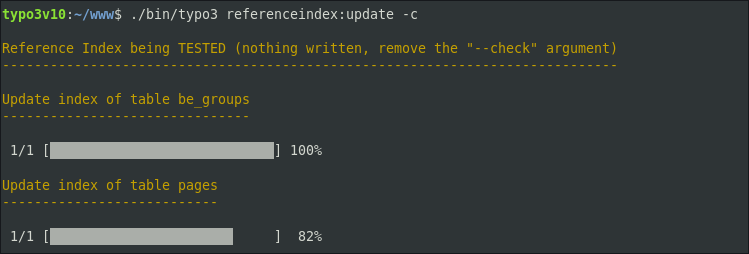
\includegraphics[width=0.85\linewidth]{InDepthChanges/82062-ProgressForReferenceIndexUpdateOnCli.png}
	\end{figure}

\end{frame}

% ------------------------------------------------------------------------------
% Feature | 59452 | scheduler:run command accepts multiple task options

\begin{frame}[fragile]
	\frametitle{Changements en profondeur}
	\framesubtitle{Planificateur}

	% decrease font size for code listing
	\lstset{basicstyle=\tiny\ttfamily}

	\begin{itemize}
		\item Il est possible d'exécuter plusieurs tâches lorsque l'option \texttt{-}\texttt{-}\texttt{task} est utilisée
	\end{itemize}

	\begin{figure}
		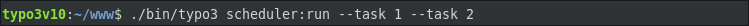
\includegraphics[width=0.85\linewidth]{InDepthChanges/59452a-MultipleTasksInSchedulerCommand.png}
	\end{figure}

	\begin{itemize}
		\item La sortie verbeuse est activée avec \texttt{-}\texttt{v} et \texttt{-}\texttt{vv}
	\end{itemize}

	\begin{figure}
		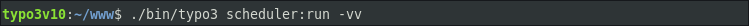
\includegraphics[width=0.85\linewidth]{InDepthChanges/59452b-MultipleTasksInSchedulerCommand.png}
	\end{figure}

\end{frame}

% ------------------------------------------------------------------------------
% Important | 18079 | pages.doktype restriction for frontend queries refined

\begin{frame}[fragile]
	\frametitle{Changements en profondeur}
	\framesubtitle{Gestion du type de page}

	\begin{itemize}
		\item La gestion interne de TYPO3 des types de page a changé.
		\item L'option \texttt{pages.doktype} définie une valeur numérique qui représente le type,
			i.e. page standard, dossier, raccourci, lien vers une url externe, etc.
		\item Les pages de certains types (i.e. dossier et corbeille) étaient exclus lorsque le contenu
			était lut depuis une page ou lors de la récupération d'enregistrements.
		\item Cette limitation est retirée et les types de valeur supérieure à 200 sont possibles.
		\item Il est conseillé aux intégrateurs et développeurs qui utilisent ces types, en TypoScript par exemple,
			de vérifier si le comportement précédent n'était pas abusé et si une mise à jour est nécessaire.
	\end{itemize}

\end{frame}

% ------------------------------------------------------------------------------
% Feature | 90203 | Make workspace available in TypoScript conditions

\begin{frame}[fragile]
	\frametitle{Changements en profondeur}
	\framesubtitle{Espaces de travail (1)}

	% decrease font size for code listing
	\lstset{basicstyle=\smaller\ttfamily}

	\begin{itemize}
		\item La variable \texttt{workspace} est introduite dans le langage des expressions.
		\item Cette variable est utilisée pour faire correspondre l'expression avec les
			paramètres communs des espaces de travail.
		\item Actuellement, ces paramètres sont supportés~:\newline
			\small
				\texttt{workspaceId}, \texttt{isLive}, et \texttt{isOffline}.
			\normalsize
		\item Par exemple~:
\begin{lstlisting}
[workspace.workspaceId === 3]
  # Current workspace ID is 3
[end]
\end{lstlisting}

	\end{itemize}

\end{frame}

% ------------------------------------------------------------------------------
% Important | 89555 | Workspace-related database records contain the proper Page ID

\begin{frame}[fragile]
	\frametitle{Changements en profondeur}
	\framesubtitle{Espaces de travail (2)}

	\begin{itemize}
		\item Depuis longtemps, le noyau de TYPO3 définissait le \texttt{pid} à \texttt{-1} pour les enregistrements non publiés.
		\item Les enregistrements versionnés sont maintenant gérés par la validation de ces trois champs~:

			\begin{itemize}
				\item \texttt{t3ver\_wsid} (l'ID de l'espace de travail de lequel l'enregistrement est versionné)
				\item \texttt{t3ver\_state} (le type de l'enregistrement versionné)
				\item \texttt{t3ver\_oid} (l'identifiant de l'enregistrement publié)
			\end{itemize}

		\item Ainsi, \texttt{pid=-1} n'est plus nécessaire.
		\item L'assistant de mise à jour converti l'ensemble des champs \texttt{pid} des enregistrements versionnés
			vers leur valeur de \texttt{pid} réelle.
		\item Les nouvelles installations ne sont pas affectées.

	\end{itemize}

\end{frame}

% ------------------------------------------------------------------------------
% Deprecation | 91030 | Runtime-Activated Packages

\begin{frame}[fragile]
	\frametitle{Changements en profondeur}
	\framesubtitle{Paquets activé à l'exécution}

	\begin{itemize}
		\item La configuration globale suivante est marquée \textbf{dépréciée}~:\newline
			\smaller
				\texttt{\$GLOBALS['TYPO3\_CONF\_VARS']['EXT']['runtimeActivatedPackages']}
			\normalsize
		\item L'usage des extensions activées à l'exécution ralenti considérablement le système.
		\item Il est conseillé aux intégrateurs de mettre en place les corrections nécessaire si un tel avertissement
			est reporté dans le journal de dépréciation~:\newline
			\begingroup
				\fontsize{8}{10}
				\texttt{Support for runtime activated packages will be removed in TYPO3 v11.0.}
			\endgroup

	\end{itemize}

\end{frame}

% ------------------------------------------------------------------------------
% Breaking | 88376 | Removed obsolete pageNotFound_handling settings

\begin{frame}[fragile]
	\frametitle{Changements en profondeur}
	\framesubtitle{Gestion de Page non trouvée}

	\begin{itemize}

		\item Les paramètres globaux suivants sont retirés~:

			\begin{itemize}
				\item {\fontsize{7}{8}\selectfont\texttt{\$GLOBALS['TYPO3\_CONF\_VARS']['FE']['pageNotFound\_handling']}}
				\item {\fontsize{7}{8}\selectfont\texttt{\$GLOBALS['TYPO3\_CONF\_VARS']['FE']['pageNotFound\_handling\_statheader']}}
				\item {\fontsize{7}{8}\selectfont\texttt{\$GLOBALS['TYPO3\_CONF\_VARS']['FE']['pageNotFound\_handling\_accessdeniedheader']}}
				\item {\fontsize{7}{8}\selectfont\texttt{\$GLOBALS['TYPO3\_CONF\_VARS']['FE']['pageUnavailable\_handling']}}
				\item {\fontsize{7}{8}\selectfont\texttt{\$GLOBALS['TYPO3\_CONF\_VARS']['FE']['pageUnavailable\_handling\_statheader']}}
			\end{itemize}

			\begin{itemize}\smaller
				\item[\ding{228}] La gestion de site mise en place en TYPO3 v9 remplace ceux-ci.
			\end{itemize}\normalsize

	\end{itemize}

\end{frame}

% ------------------------------------------------------------------------------
% Important | 87980 | Page Is Being Generated Message Has Been Removed

\begin{frame}[fragile]
	\frametitle{Changements en profondeur}
	\framesubtitle{Gestion de Page non trouvée}

	\begin{itemize}

		\item Le message «~\textit{Page is being generated}~» et la réponse temporaire
			HTTP 503 correspondante ont été retirés.
	\end{itemize}

	\begin{figure}
		
\includegraphics[width=0.70\linewidth]{InDepthChanges/87980-PageIsBeingGenerated.png}
	\end{figure}

	\begin{itemize}
		\item Au lieu de se décharger de l'attente pour le contenu final de la page,
			les requêtes simultanées attendent le rendu du contenu réel de la page.
	\end{itemize}

\end{frame}

% ------------------------------------------------------------------------------
% Feature | 84262 | Update EXT:felogin to Extbase (long-term goal, not completed yet)
% Breaking | 88706 | Streamline felogin locallang keys
% Breaking | 88129 | Renamed felogin flexform fields

\begin{frame}[fragile]
	\frametitle{Changements en profondeur}
	\framesubtitle{Connexion Frontend~: Extbase}

	\begin{itemize}
		\item Le formulaire de connexion frontend (\texttt{EXT:felogin}) est convertit vers Extbase et Fluid.

		\item Les changements suivants sont implémentés~:

		\begin{itemize}
			\item[\ding{202}] Le préfixe «~\texttt{ll\_}~» est retiré des clés locallang.

				\begin{itemize}
					\item[\ding{228}] Mettez à jour votre TypoScript si vous avez surchargé les libellés de langue et effacez le préfixe «~\texttt{ll\_}~» de vos clés.
				\end{itemize}

			\item[\ding{203}] La structure des FlexForms est remaniée.

				\begin{itemize}
					\item[\ding{228}] Exécutez l'assistant de mise à jour pour migrer les valeurs des FlexForm.
				\end{itemize}

		\end{itemize}

	\end{itemize}

\end{frame}

% ------------------------------------------------------------------------------
% Breaking | 88583 | Database field sys_language.static_lang_isocode removed
% Deprecation | 88567 | $GLOBALS['LOCAL_LANG']

\begin{frame}[fragile]
	\frametitle{Changements en profondeur}
	\framesubtitle{Langues}

	\begin{itemize}
		\item Codes ISO~:

			\begin{itemize}
				\item Le champ inutilisé de base de données \texttt{static\_lang\_isocode} est retiré.
				\item \texttt{EXT:static\_info\_tables} peut être installée pour le rétablir si requis.
				\item Il est conseillé aux développeurs de récupérer toutes les métadonnées d'une langue
					en utilisation la configuration de site et l'API SiteLanguage.
			\end{itemize}

		\item Fichiers de langue~:

			\begin{itemize}
				\item Le tableau global \texttt{\$GLOBALS[LOCAL\_LANG]} est déprécié.
				\item Les 2ième et 3ième arguments de \texttt{LanguageService->includeLLFile()} sont dépréciés.
			\end{itemize}

	\end{itemize}

\end{frame}

% ------------------------------------------------------------------------------
% Feature | 88643 | New Mail API based on symfony/mailer and symfony/mime
% Breaking | 88643 | Removed Swiftmailerswiftmailer Dependency

\begin{frame}[fragile]
	\frametitle{Changements en profondeur}
	\framesubtitle{Nouvelle API Mail}

	\begin{itemize}
		\item SwiftMailer est remplacé par des bibliothèques plus modernes~:

			\begin{itemize}
				\item \texttt{symfony/mime} pour la création de messages
				\item \texttt{symfony/mailer} pour l'envoi de mails
			\end{itemize}

		\item La fonction PHP \texttt{mail()} n'est plus supportée.

			\begin{itemize}\smaller
				\item[\ding{228}] Il est recommandé de passer sur \texttt{sendmail} ou \texttt{smtp}.
			\end{itemize}\normalsize

		\item Les plugins ou les transports pour SwiftMailer personnalisés nécessiteront une migration.

		\item Voir la \href{https://symfony.com/doc/current/mailer.html}{documentation de Symfony (en)}
			pour plus d'informations sur l'utilisation des capacités de la nouvelle API Mail.
	\end{itemize}

\end{frame}

% ------------------------------------------------------------------------------
% ...

\begin{frame}[fragile]
	\frametitle{Changements en profondeur}
	\framesubtitle{Normes PSR}

	\begin{itemize}
		\item TYPO3 v10 LTS suit ces \href{https://www.php-fig.org/psr/}{normes PSR (en)}~:
			\vspace{0.2cm}
			\begin{itemize}
				\item PSR-0 / PSR-4\tabto{3.7cm}Chargement automatique
				\item PSR-1 / PSR-2\tabto{3.7cm}Guide de développement
				\item PSR-3\tabto{3.7cm}Journalisation
				\item PSR-7 / PSR-15 / PSR-17\tabto{3.7cm}Prise en charge des requêtes et réponses HTTP)
				\item PSR-11\tabto{3.7cm}Injection de dépendances (Conteneur de service)
				\item PSR-14\tabto{3.7cm}Gestionnaire d'événements
				\item PSR-18\tabto{3.7cm}Client HTTP
			\end{itemize}

	\end{itemize}

\end{frame}

% ------------------------------------------------------------------------------
% Feature | 88799 | Use PSR-3 interface for logging

\begin{frame}[fragile]
	\frametitle{Changements en profondeur}
	\framesubtitle{Interface de journalisation PSR-3}

	\begin{itemize}
		\item Le framework de journalisation de TYPO3 (en particulier LogLevel et LogManager)
			implémente l'\href{https://www.php-fig.org/psr/psr-3/}{interface de journalisation PSR-3 (en)}.

		\item PSR-3 est une méthode standardisée permettant aux bibliothèques de recevoir un objet
			\texttt{Psr\textbackslash
				Log\textbackslash
				LoggerInterface} et d'écrire des journaux de façon simple et universelle.

			\item Ceci permet aux développeurs d'utiliser des journaliseurs personnalisés et d'interagir
				avec d'autres systèmes de journalisation.

	\end{itemize}

\end{frame}

% ------------------------------------------------------------------------------
% Feature | 84112 | Symfony dependency injection for core and Extbase

\begin{frame}[fragile]
	\frametitle{Changements en profondeur}
	\framesubtitle{Injection et gestion de dépendances Symfony (1)}

	\begin{itemize}
		\item Le paquet \texttt{symfony/dependency-injection} est intégré et utilisé pour gérer
			les dépendances à travers le système et l'injection de dépendances pour les classes.

		\item Cette approche vise à remplacer l'injection de dépendances d'Extbase

		\item Ainsi, les classes doivent être ajustées et il faut éviter (lorsque possible)~:

			\begin{itemize}\small
				\item \texttt{\textbackslash
					TYPO3\textbackslash
					CMS\textbackslash
					Extbase\textbackslash
					Object\textbackslash
					ObjectManager}
				\item \texttt{\textbackslash
					TYPO3\textbackslash
					CMS\textbackslash
					Core\textbackslash
					Utility\textbackslash
					GeneralUtility::makeInstance()}
			\end{itemize}\normalsize

	\end{itemize}

\end{frame}

% ------------------------------------------------------------------------------
% Feature | 84112 | Symfony dependency injection for core and Extbase

\begin{frame}[fragile]
	\frametitle{Changements en profondeur}
	\framesubtitle{Injection et gestion de dépendances Symfony (2)}

	% decrease font size for code listing
	\lstset{basicstyle=\tiny\ttfamily}

	\begin{itemize}
		\item Les options de configuration incluent~:

			\begin{itemize}
				\item L'association automatique «~autowiring~» (voir l'exemple ci-dessous)
				\item L'association manuelle
					(voir \href{https://docs.typo3.org/c/typo3/cms-core/master/en-us/Changelog/10.0/Feature-84112-SymfonyDependencyInjectionForCoreAndExtbase.html}{journal des changements (en)})
				\item Fonctionnalités avancées
					(voir \href{https://docs.typo3.org/c/typo3/cms-core/master/en-us/Changelog/10.0/Feature-84112-SymfonyDependencyInjectionForCoreAndExtbase.html}{journal des changements (en)})
			\end{itemize}
\begin{lstlisting}
# Configuration/Services.yaml
services:
  _defaults:
    autowire: true
    autoconfigure: true
    public: false

  Your\Namespace\:
    resource: '../Classes/*'
\end{lstlisting}

		\item Voir la \href{https://symfony.com/doc/current/service_container.html}{documentation de Symfony (en)} pour plus d'informations.

	\end{itemize}

\end{frame}

% ------------------------------------------------------------------------------
% Feature | 88769 | Introduce a generic EventDispatcher based on PSR-14
% Feature | 88770 | Add PSR-14 EventDispatcher logic based on DI

\begin{frame}[fragile]
	\frametitle{Changements en profondeur}
	\framesubtitle{Gestionnaire d'événements (1)}

	\begin{itemize}
		\item Un nouveau système «~EventDispatcher~» est ajouté pour remplacer les Hooks et
			les concepts de Signal/Slot.

		\item Ce système est basé sur la \href{https://www.php-fig.org/psr/psr-14}{norme PSR-14 (en)}
			permettant aux développeurs d'injecter des comportement dans l'application de façon
			simple et systématique.

		\item PSR-14 contient quatre composants~:

			\begin{itemize}
				\item Un objet \textbf{EventDispatcher} permettant de déclencher un événement.
				\item Un objet \textbf{ListenerProvider} contenant les écouteurs enregistrés pour
					tous les événements.
				\item Un ou plusieurs objets \textbf{Event} qui sont appelés depuis le cœur de TYPO3
					ou les extensions («~Émetteurs~»)
				\item Un ou plusieurs objets \textbf{Listeners} (habituellement dans les extensions
					ou les paquets PHP) qui sont enregistrés.
			\end{itemize}

% Short-Term goal is to deprecate SignalSlot dispatcher in TYPO3 v10,
% and migrate all signals to the EventDispatcher.

	\end{itemize}

\end{frame}

% ------------------------------------------------------------------------------
% Feature | 88769 | Introduce a generic EventDispatcher based on PSR-14
% Feature | 88770 | Add PSR-14 EventDispatcher logic based on DI

\begin{frame}[fragile]
	\frametitle{Changements en profondeur}
	\framesubtitle{Gestionnaire d'événements (2)}

	% decrease font size for code listing
	\lstset{basicstyle=\tiny\ttfamily}

	Exemple d'implémentation

	\begin{itemize}\smaller
		\item[\ding{202}] Ajoutez la balise \texttt{event.listener} au fichier \texttt{Configuration/Services.yaml}~:
\begin{lstlisting}
services:
  Vendor\Example\EventListener\NullMailer:
    tags:
      - { name: event.listener, identifier: 'myListener', event: TYPO3\CMS\Core\Mail\Event\AfterMailerInitializationEvent, before: 'redirects, anotherIdentifier' }
\end{lstlisting}

		\item[\ding{203}] Implémentez votre objet événement~:
\begin{lstlisting}
namespace Vendor\Example\EventListener;

class NullMailer
{
  public function __invoke(AfterMailerInitializationEvent \$event): void
  {
    \$event->getMailer()->injectMailSettings(['transport' => 'null']);
  }
}
\end{lstlisting}

	\end{itemize}\normalsize

\end{frame}

% ------------------------------------------------------------------------------
% Feature | 88769 | Introduce a generic EventDispatcher based on PSR-14
% Feature | 88770 | Add PSR-14 EventDispatcher logic based on DI

\begin{frame}[fragile]
	\frametitle{Changements en profondeur}
	\framesubtitle{Gestionnaire d'événements (3)}

	% decrease font size for code listing
	\lstset{basicstyle=\tiny\ttfamily}

	\begin{itemize}
		\item La liste des écouteurs d'événements (\textit{Event Listeners}) est disponible en Backend~:\newline
			\smaller
				(l'extension \texttt{EXT:lowlevel} est nécessaire)
			\normalsize
	\end{itemize}

	\begin{figure}
		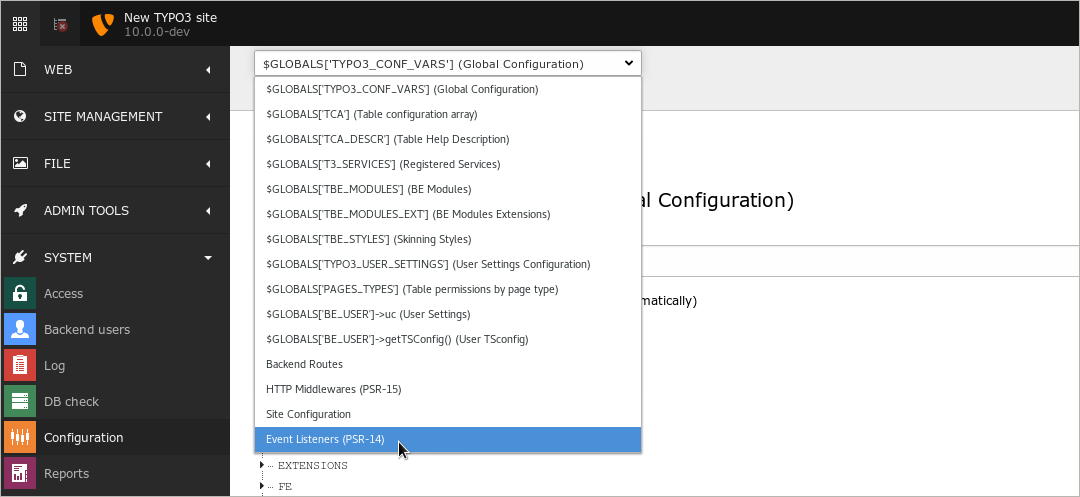
\includegraphics[width=0.70\linewidth]{InDepthChanges/88770-PSR14-EventDispatcher.png}
	\end{figure}

\end{frame}

% ------------------------------------------------------------------------------
% Feature | 88769 | Introduce a generic EventDispatcher based on PSR-14
% Feature | 88770 | Add PSR-14 EventDispatcher logic based on DI

\begin{frame}[fragile]
	\frametitle{Changements en profondeur}
	\framesubtitle{Gestionnaire d'événements (4)}

	% decrease font size for code listing
	\lstset{basicstyle=\tiny\ttfamily}

	\begin{itemize}
		\item Bonnes pratiques~:

			\begin{itemize}
				\item N'implémentez qu'un seul écouteur par classe PHP et utilisez \texttt{\_\_invoke()}
					comme nom de méthode.
				\item Ajouter le suffixe «~\texttt{Event}~» au nom des classes PHP d'événement
					lors de leur création.
				\item Placez la classe événement dans un dossier approprié, i.e. \texttt{Classes/Database/Event}.
				\item Utilisez la forme constructeur de l'injection de dépendances pour recevoir
					l'objet EventDispatcher si possible.
			\end{itemize}

		\item Remarque supplémentaire~:\newline
			\small
				Les événement fournit par le cœur TYPO3 respectent la politique de dépréciation,
				sauf pour le constructeur dont les arguments peuvent changer.
			\normalsize

	\end{itemize}

\end{frame}

% ------------------------------------------------------------------------------
% Feature | 90265 | Show dispatched Events in Admin Panel

\begin{frame}[fragile]
	\frametitle{Changements en profondeur}
	\framesubtitle{Événements PSR-14 dans le panneau d'administration}

	\begin{itemize}
		\item Le panneau d'administration affiche tous les événements PSR-14
			qui ont été déclenchés dans la requête courante.
	\end{itemize}

	\begin{figure}
		
\includegraphics[width=0.85\linewidth]{InDepthChanges/90265-ShowDispatchedEventsInAdminPanel.png}
	\end{figure}

\end{frame}

% ------------------------------------------------------------------------------
% Feature | 89018 | Provide implementation for PSR-17 HTTP Message Factories

\begin{frame}[fragile]
	\frametitle{Changements en profondeur}
	\framesubtitle{Fabriques de messages HTTP PSR-17}

	\begin{itemize}
		\item L'implémentation des fabriques de messages HTTP
			\href{https://www.php-fig.org/psr/psr-17/}{PSR-17} est ajoutée.
		\item Les interfaces de fabrique de messages HTTP devraient être
			utilisées comme dépendance des gestionnaires de requête ou services
			créant des objet message PSR-7.
		\item PSR-17 consiste en six interfaces de fabrique~:

			\begin{itemize}\smaller
				\item \texttt{\textbackslash
					Psr\textbackslash
					Http\textbackslash
					Message\textbackslash
					RequestFactoryInterface}
				\item \texttt{\textbackslash
					Psr\textbackslash
					Http\textbackslash
					Message\textbackslash
					ResponseFactoryInterface}
				\item \texttt{\textbackslash
					Psr\textbackslash
					Http\textbackslash
					Message\textbackslash
					ServerRequestFactoryInterface}
				\item \texttt{\textbackslash
					Psr\textbackslash
					Http\textbackslash
					Message\textbackslash
					StreamFactoryInterface}
				\item \texttt{\textbackslash
					Psr\textbackslash
					Http\textbackslash
					Message\textbackslash
					UploadedFileFactoryInterface}
				\item \texttt{\textbackslash
					Psr\textbackslash
					Http\textbackslash
					Message\textbackslash
					UriFactoryInterface}

			\end{itemize}\normalsize

		\item Voir la
			\href{https://docs.typo3.org/c/typo3/cms-core/master/en-us/Changelog/10.1/Feature-89018-ProvideImplementationForPSR-17HTTPMessageFactories.html}{documentation (en)}
			pour des exemples de code.

	\end{itemize}

\end{frame}

% ------------------------------------------------------------------------------
% Feature | 89216 | PSR-18 HTTP Client Implementation

\begin{frame}[fragile]
	\frametitle{Changements en profondeur}
	\framesubtitle{Client HTTP PSR-18}

	\begin{itemize}
		\item L'implémentation du client HTTP
			\href{https://www.php-fig.org/psr/psr-18/}{PSR-18} est ajoutée.
		\item Elle permet de générer des requêtes basées sur des objets message
			PSR-7 sans dépendre d'une implémentation de client HTTP spécifique.
		\item Ça ne remplace pas l'actuelle encapsulation de \href{http://guzzlephp.org/}{Guzzle},
			mais fournie une alternative plus générique.
		\item PSR-18 consiste en une interface de client et trois interfaces d'exception~:

			\begin{itemize}\smaller
				\item \texttt{\textbackslash
					Psr\textbackslash
					Http\textbackslash
					Client\textbackslash
					ClientInterface}
				\item \texttt{\textbackslash
					Psr\textbackslash
					Http\textbackslash
					Client\textbackslash
					ClientExceptionInterface}
				\item \texttt{\textbackslash
					Psr\textbackslash
					Http\textbackslash
					Client\textbackslash
					NetworkExceptionInterface}
				\item \texttt{\textbackslash
					Psr\textbackslash
					Http\textbackslash
					Client\textbackslash
					RequestExceptionInterface}
			\end{itemize}\normalsize

		\item Voir la
			\href{https://docs.typo3.org/c/typo3/cms-core/master/en-us/Changelog/10.1/Feature-89216-PSR-18HTTPClientImplementation.html}{documentation (en)}
			pour un exemple de code.

	\end{itemize}

\end{frame}

% ------------------------------------------------------------------------------
% Breaking | 88182 | jsfunc.inline.js has been dropped
% Breaking | 88427 | jsfunc.evalfield.js has been removed
% Breaking | 88667 | Removed additionalJavaScriptSubmit from FormEngine
% Deprecation | 88433 | Deprecate top.openUrlInWindow

\begin{frame}[fragile]
	\frametitle{Changements en profondeur}
	\framesubtitle{Options et fonctions JavaScript (1)}

	\begin{itemize}
		\item Les fichiers JavaScript suivants ont été retirés~:

			\begin{itemize}
				\item \texttt{jsfunc.inline.js}
				\item \texttt{jsfunc.evalfield.js}
			\end{itemize}

			\begin{itemize}\smaller
				\item[\ding{228}] Utilisez plutôt \texttt{TYPO3/CMS/Backend/FormEngineValidation}.
			\end{itemize}\normalsize

		\item Des gestionnaires de soumission additionnels pouvaient être ajoutés avec l'option
			\texttt{additionalJavaScriptSubmit}. Elle est retirée.

			\begin{itemize}\smaller
				\item[\ding{228}] À la place, créez et inscrivez un module AMD\@.
			\end{itemize}\normalsize

		\item La fonction JavaScript globale \texttt{top.openUrlInWindow()} est marquée dépréciée.

	\end{itemize}

\end{frame}

% ------------------------------------------------------------------------------
% Breaking | 88411 | TBE_EDITOR.typo3form removed
% Deprecation | 88432 | Replaced md5js with an AMD module
% Deprecation | 88428 | top.rawurlencode and top.str_replace
% Deprecation | 88651 | Replace TYPO3/CMS/Backend/SplitButtons with TYPO3/CMS/Backend/DocumentSaveActions

\begin{frame}[fragile]
	\frametitle{Changements en profondeur}
	\framesubtitle{Options et fonctions JavaScript (2)}

	\begin{itemize}

		\item L'objet global \texttt{TBE\_EDITOR.typo3form} ainsi que \texttt{typo3FormFieldSet}
			et \texttt{typo3FormFieldGet} sont retirés.

		\item Le fichier \texttt{md5.js} est marqué déprécié.

			\begin{itemize}\smaller
				\item[\ding{228}] À la place, chargez le module AMD \texttt{TYPO3/CMS/Backend/Hashing/Md5} via RequireJS\@.
			\end{itemize}\normalsize

		\item Les fonctions globales JavaScript suivantes sont marquées dépréciées~:

		\begin{itemize}
			\item \texttt{top.rawurlencode()}
			\item \texttt{top.str\_replace()}
		\end{itemize}

		\item Le module \texttt{TYPO3/CMS/Backend.SplitButtons} est déprécié.

			\begin{itemize}\smaller
				\item[\ding{228}] Utilisez plutôt \texttt{TYPO3/CMS/Backend/DocumentSaveActions}.
			\end{itemize}\normalsize

 	\end{itemize}

\end{frame}

% ------------------------------------------------------------------------------
% Important | 87894 | Removed PHP Dependency algo26-matthiasidna-convert

\begin{frame}[fragile]
	\frametitle{Changements en profondeur}
	\framesubtitle{Domaines en UTF-8}

	\begin{itemize}
		\item PHP possède des fonctions natives de conversion d'un domaine de l'UTF-8 en forme IDNA ASCII
			(«~punicode~»), par exemple \href{https://www.php.net/manual/en/function.idn-to-ascii.php}{idn\_to\_ascii()}.

		\item Elles sont utilisées directement lorsque l'extension PHP
			«~\href{https://www.php.net/manual/en/book.intl.php}{intl}~» est installée.

		\item Si l'extension PHP n'est pas installée, le paquet \texttt{symfony/polyfill-intl-idn}
			fournit ces fonctions.

		\item Le paquet \texttt{algo26-matthias/idna-convert} qui était utilisé auparavant est retiré.

	\end{itemize}

\end{frame}

% ------------------------------------------------------------------------------
% Feature | 87665 | Introduce BitSet class

\begin{frame}[fragile]
	\frametitle{Changements en profondeur}
	\framesubtitle{Classe BitSet}

	% decrease font size for code listing
	\lstset{basicstyle=\tiny\ttfamily}

	\begin{itemize}
		\item Une classe pour gérer efficacement les indicateurs booléens est introduite~:\newline
			\texttt{TYPO3\textbackslash
				CMS\textbackslash
				Core\textbackslash
				Type\textbackslash
				BitSet}

		\item Par example~:
\begin{lstlisting}
define('PERMISSIONS_NONE', 0b0); // 0
define('PERMISSIONS_PAGE_SHOW', 0b1); // 1
define('PERMISSIONS_PAGE_EDIT', 0b10); // 2
define('PERMISSIONS_PAGE_DELETE', 0b100); // 4
define('PERMISSIONS_PAGE_NEW', 0b1000); // 8
define('PERMISSIONS_CONTENT_EDIT', 0b10000); // 16
define('PERMISSIONS_ALL', 0b11111); // 31

\$bitSet = new \TYPO3\CMS\Core\Type\BitSet(PERMISSIONS_PAGE_SHOW | PERMISSIONS_PAGE_NEW);
\$bitSet->get(PERMISSIONS_PAGE_SHOW); // true
\$bitSet->get(PERMISSIONS_CONTENT_EDIT); // false
\end{lstlisting}

	\end{itemize}

\end{frame}

% ------------------------------------------------------------------------------
% Important | 87516 | Remove Core HTTP Request Handler Interface

\begin{frame}[fragile]
	\frametitle{Changements en profondeur}
	\framesubtitle{Gestionnaire de requêtes (1)}

	\begin{itemize}
		\item L'interface interne suivante est retirée en faveur du gestionnaire de requête PSR-15
			et des middlewares~:\newline
			\texttt{TYPO3\textbackslash
				CMS\textbackslash
				Core\textbackslash
				Http\textbackslash
				RequestHandlerInterface}

	\end{itemize}

\end{frame}

% ------------------------------------------------------------------------------
% Breaking | 88687 | Configure extbase request handlers via PHP

\begin{frame}[fragile]
	\frametitle{Changements en profondeur}
	\framesubtitle{Gestionnaire de requêtes (2)}

	% decrease font size for code listing
	\lstset{basicstyle=\tiny\ttfamily}

	\begin{itemize}
		\item La configuration du gestionnaire de requêtes Extbase ne s'effectue plus en TypoScript.

		\smaller\textbf{Ancienne} méthode par TypoScript~:\normalsize
\begin{lstlisting}
config.tx_extbase {
  mvc {
    requestHandlers {
      Vendor\Example\Mvc\Web\FrontendRequestHandler = Vendor\Example\Mvc\Web\FrontendRequestHandler
    }
  }
}
\end{lstlisting}

		\smaller\textbf{Nouvelle} Méthode par le fichier \texttt{Configuration/Extbase/RequestHandlers.php}~:\normalsize
\begin{lstlisting}
<?php
declare(strict_types = 1);

return [
  \Vendor\Example\Mvc\Web\FrontendRequestHandler::class,
];
\end{lstlisting}

	\end{itemize}

\end{frame}

% ------------------------------------------------------------------------------
% Deprecation | 87550 | Use controller classes when registering plugins/modules

\begin{frame}[fragile]
	\frametitle{Changements en profondeur}
	\framesubtitle{Extbase et Fluid (1)}

	% decrease font size for code listing
	\lstset{basicstyle=\tiny\ttfamily}

	\begin{itemize}
		\item L'inscription des plugins/modules nécessite les noms qualifiés des classes~:

			\begin{itemize}\smaller
				\item \texttt{\textbackslash
					TYPO3\textbackslash
					CMS\textbackslash
					Extbase\textbackslash
					Utility\textbackslash
					ExtensionUtility::configurePlugin()}
				\item \texttt{\textbackslash
					TYPO3\textbackslash
					CMS\textbackslash
					Extbase\textbackslash
					Utility\textbackslash
					ExtensionUtility::registerModule()}
			\end{itemize}\normalsize

		\item Aussi, ne plus spécifier le nom de fournisseur avec le nom d'extension (premier argument).

			\begin{itemize}\smaller
				\item[\ding{228}] Utilisez «~\texttt{ExampleBlog}~» au lieu de «~\texttt{Vendor.ExampleBlog}~».
			\end{itemize}

		\item Exemple~:
\begin{lstlisting}
\TYPO3\CMS\Extbase\Utility\ExtensionUtility::configurePlugin(
  'ExampleBlog', // previously: 'Vendor.ExampleBlog'
  'pi1',
  [
    \Vendor\Example\Controller\BlogController::class => 'list,update,delete'
  ],
  [
    \Vendor\Example\Controller\BlogController::class => 'list,update,delete'
  ]
);
\end{lstlisting}

	\end{itemize}

\end{frame}

% ------------------------------------------------------------------------------
% Breaking | 87627 | Remove Property extensionName of AbstractController

\begin{frame}[fragile]
	\frametitle{Changements en profondeur}
	\framesubtitle{Extbase et Fluid (2)}

	\begin{itemize}
		\item La propriété \texttt{extensionName} de AbstractController est retirée.

			\begin{itemize}\smaller
				\item[\ding{228}] Utilisez alors \texttt{\textbackslash
					TYPO3\textbackslash
					CMS\textbackslash
					Extbase\textbackslash
					Mvc\textbackslash
					Request::getControllerExtensionName()}.
			\end{itemize}\normalsize

	\end{itemize}

\end{frame}

% ------------------------------------------------------------------------------
% Feature | 87457 | Use symfony/propertyinfo to gather doc block information

\begin{frame}[fragile]
	\frametitle{Changements en profondeur}
	\framesubtitle{Extbase et Fluid (3)}

	% decrease font size for code listing
	\lstset{basicstyle=\tiny\ttfamily}

	\begin{itemize}
		\item Les modèles Extbase supportent les noms de classe non qualifiés dans le bloc de documentation.
\begin{lstlisting}
use TYPO3\CMS\Extbase\Persistence\ObjectStorage;
use ExtbaseTeam\BlogExample\Domain\Model\Comment;

class Post
{
  /**
   * @var ObjectStorage<Comment>
   */
  public \$comments;
}
\end{lstlisting}

	\end{itemize}

\end{frame}

% ------------------------------------------------------------------------------
% Breaking | 87957 | Validators are not registered automatically in Extbase anymore

\begin{frame}[fragile]
	\frametitle{Changements en profondeur}
	\framesubtitle{Extbase et Fluid (4)}

	% decrease font size for code listing
	\lstset{basicstyle=\tiny\ttfamily}

	\begin{itemize}
		\item Les validateurs ne sont plus inscrits automatiquement dans Extbase.
		\item Pour un modèle nommé
			\small\texttt{Vendor\textbackslash
				Example\textbackslash
				Domain\textbackslash
				Model\textbackslash
				Blog}\normalsize,\newline
			Extbase utilisait automatiquement le validateur
			\small\texttt{Vendor\textbackslash
				Example\textbackslash
				Domain\textbackslash
				Validator\textbackslash
				BlogValidator}\normalsize

		\item Les validateurs doivent être inscrits manuellement~:
\begin{lstlisting}
use Vendor\Example\Domain\Model\Blog;
use TYPO3\CMS\Extbase\Annotation as Extbase;
use TYPO3\CMS\Extbase\Mvc\Controller\ActionController;

class BlogController extends ActionController
{
  /**
   * @Extbase\Validate(param="blog", validator="Vendor\Example\Domain\Validator\BlogValidator")
   */
  public function showAction(Blog \$blog)
  {
    // ...
  }
}
\end{lstlisting}

	\end{itemize}

\end{frame}

% ------------------------------------------------------------------------------
% Breaking | 87594 | Harden Extbase

\begin{frame}[fragile]
	\frametitle{Changements en profondeur}
	\framesubtitle{Extbase et Fluid (5)}

	% decrease font size for code listing
	\lstset{basicstyle=\smaller\ttfamily}

	\begin{itemize}
		\item Les fichiers de classe utilisent le mode «~types stricts~» et les indications de type scalaires.
\begin{lstlisting}
<?php
declare(strict_types=1);
\end{lstlisting}

		% Method signatures in Extbase classes have been updated.
		\item Ceci lève des erreurs PHP fatales lorsque les signatures de méthode dans les extensions
			ne sont pas compatibles avec l'interface ou la classe parente.

		\item Voir \href{https://forge.typo3.org/issues/87594}{forge \#87594 (en)}
			pour la liste complète des fichiers et leurs changements.

		\item Cette tâche est toujours en cours et de nouveaux changements seront effectués.

	\end{itemize}

\end{frame}

% ------------------------------------------------------------------------------
% Feature | 88995 | Calling registerPlugin with vendor name

\begin{frame}[fragile]
	\frametitle{Changements en profondeur}
	\framesubtitle{Extbase et Fluid (6)}

	% decrease font size for code listing
	\lstset{basicstyle=\smaller\ttfamily}

	\begin{itemize}
		\item Omettez le nom de fournisseur lors de l'inscription d'un plugin avec\newline
			\smaller
				\texttt{\textbackslash
					TYPO3\textbackslash
					CMS\textbackslash
					Extbase\textbackslash
					Utility\textbackslash
					ExtensionUtility::registerPlugin()}
			\normalsize

		\item Par exemple, utilisez «~\texttt{Form}~» au lieu de «~\texttt{TYPO3.CMS.Form}~»\newline
			\small(premier paramètre)\normalsize
\begin{lstlisting}
\TYPO3\CMS\Extbase\Utility\ExtensionUtility::registerPlugin(
  'Form',
  'Formframework',
  'Form',
  'content-form',
);
\end{lstlisting}

	\end{itemize}

\end{frame}

% ------------------------------------------------------------------------------
% Feature | 89870 | New PSR-14 Events for Extbase-related signals

\begin{frame}[fragile]
	\frametitle{Changements en profondeur}
	\framesubtitle{Extbase et Fluid (7)}

	% decrease font size for code listing
	\lstset{basicstyle=\tiny\ttfamily}

	\begin{itemize}
		\item Les événements suivants basés sur PSR-14 sont introduits pour des signaux Extbase~:
\begin{lstlisting}
TYPO3\CMS\Extbase\Event\Mvc\AfterRequestDispatchedEvent
TYPO3\CMS\Extbase\Event\Mvc\BeforeActionCallEvent
TYPO3\CMS\Extbase\Event\Persistence\AfterObjectThawedEvent
TYPO3\CMS\Extbase\Event\Persistence\ModifyQueryBeforeFetchingObjectDataEvent
TYPO3\CMS\Extbase\Event\Persistence\ModifyResultAfterFetchingObjectDataEvent
TYPO3\CMS\Extbase\Event\Persistence\EntityAddedToPersistenceEvent
TYPO3\CMS\Extbase\Event\Persistence\EntityFinalizedAfterPersistenceEvent
TYPO3\CMS\Extbase\Event\Persistence\EntityUpdatedInPersistenceEvent
TYPO3\CMS\Extbase\Event\Persistence\EntityRemovedFromPersistenceEvent
TYPO3\CMS\Extbase\Event\Persistence\EntityPersistedEvent
\end{lstlisting}

		\item Les signaux existants sont remplacés et ne doivent plus être utilisés.

	\end{itemize}

\end{frame}

% ------------------------------------------------------------------------------
% Breaking | 87623 | Replace config.persistence.classes typoscript configuration (1)

\begin{frame}[fragile]
	\frametitle{Changements en profondeur}
	\framesubtitle{Extbase et Fluid (8) - Class Mapping (1)}

	% decrease font size for code listing
	\lstset{basicstyle=\tiny\ttfamily}

	\begin{itemize}
		\item La définition des associations entre champs et propriétés de la persistance en TypoScript
			n'est plus supportée~:
\begin{lstlisting}
config.tx_example_blog {
  persistence {
    classes {
      Vendor\Example\Domain\Model\Author {
        mapping {
          tableName = fe_users
          columns.name.mapOnProperty = fullname
        }
      }
    }
  }
}
\end{lstlisting}

	\end{itemize}

\end{frame}

% ------------------------------------------------------------------------------
% Breaking | 87623 | Replace config.persistence.classes typoscript configuration (2)

\begin{frame}[fragile]
	\frametitle{Changements en profondeur}
	\framesubtitle{Extbase et Fluid (9) - Class Mapping (2)}

	% decrease font size for code listing
	\lstset{basicstyle=\tiny\ttfamily}

	\begin{itemize}
		\item Les associations entre les modèles et la base doivent être indiquées dans le fichier
			\texttt{Configuration/Extbase/Persistence/Classes.php}~:
\begin{lstlisting}
<?php
declare(strict_types = 1);

return [
  \Vendor\Example\Domain\Model\Author::class => [
    'tableName' => 'fe_users',
    'properties' => [
      'fullname' => [
        'fieldName' => 'name'
      ]
    ]
  ]
];
\end{lstlisting}

		\begin{itemize}\smaller
			\item[\ding{228}] NB~: le nom de la propriété et le champ de base de données ont été interchangés~!\newline
				Avant~:\tabto{1.6cm}\texttt{<db-field>.mapOnProperty = <property>}\newline
				Maintenant~:\tabto{1.6cm}\texttt{properties.<property>.fieldname = <db-field>}
		\end{itemize}\normalsize

	\end{itemize}

\end{frame}

% ------------------------------------------------------------------------------
% Deprecation | 88406 | setCacheHash/noCacheHash options in ViewHelpers and UriBuilder

\begin{frame}[fragile]
	\frametitle{Changements en profondeur}
	\framesubtitle{cHash dans l'UriBuilder et les ViewHelpers}

	% decrease font size for code listing
	\lstset{basicstyle=\smaller\ttfamily}

	\begin{itemize}
		\item Les deux méthodes d'UriBuilder suivantes sont dépréciées~:

			\begin{itemize}
				\item \texttt{UriBuilder->setUseCacheHash()}
				\item \texttt{UriBuilder->getUseCacheHash()}
			\end{itemize}

		\item Ce qui impact de nombreux ViewHelpers Fluid~:
	\end{itemize}
	\begin{columns}[T]
		\begin{column}{.05\textwidth}
		\end{column}
		\begin{column}{.45\textwidth}
			\begin{itemize}\smaller
				\item \texttt{f:form}
				\item \texttt{f:link.action}
				\item \texttt{f:link.page}
				\item \texttt{f:link.typolink}
				\item \texttt{f:uri.action}
			\end{itemize}\normalsize
		\end{column}
		\begin{column}{.45\textwidth}
			\begin{itemize}\smaller
				\item \texttt{f:uri.page}
				\item \texttt{f:uri.typolink}
				\item \texttt{f:widget.link}
				\item \texttt{f:widget.uri}
			\end{itemize}\normalsize
		\end{column}
	\end{columns}
	\vspace{0.2cm}
	\begin{itemize}
		\item \ldots comme l'option TypoScript «~\texttt{useCacheHash}~».
	\end{itemize}

\end{frame}

% ------------------------------------------------------------------------------
% Feature | 86967 | Allow fetching uid of a LazyLoadingProxy without loading the object first

\begin{frame}[fragile]
	\frametitle{Changements en profondeur}
	\framesubtitle{Mandataire de chargement différé}

	% decrease font size for code listing
	\lstset{basicstyle=\tiny\ttfamily}

	\begin{itemize}
		\item La méthode \texttt{getUid()} est ajoutée à la classe\newline
			\texttt{TYPO3\textbackslash
				CMS\textbackslash
				Extbase\textbackslash
				Persistence\textbackslash
				Generic\textbackslash
				LazyLoadingProxy}.
		\item Les développeurs peuvent donc récupérer l'identifiant d'un objet utilisant un mandataire
			sans devoir récupérer celui-ci depuis la base de données.

	\end{itemize}

\end{frame}

% ------------------------------------------------------------------------------
% Feature | 89644 | Add optional argument fields to editRecord ViewHelpers

\begin{frame}[fragile]
	\frametitle{Changements en profondeur}
	\framesubtitle{ViewHelper \texttt{editRecord}}

	% decrease font size for code listing
	\lstset{basicstyle=\tiny\ttfamily}

	\begin{itemize}
		\item L'argument optionnel \texttt{fields} est ajouté aux ViewHelpers
			\texttt{uri.editRecord} et \texttt{link.editRecord}.
		\item Si défini, le moteur de formulaire créé un formulaire pour éditer
			uniquement les champs spécifiés
		\item L'exemple suivant génère un lien pour éditer le champs \texttt{tt\_content.bodytext}
			de l'enregistrement avec l'identifiant 42.
\begin{lstlisting}
<be:link.editRecord uid="42" table="tt_content" fields="bodytext" returnUrl="foo/bar">
  Edit record
</be:link.editRecord>
\end{lstlisting}

	\end{itemize}

\end{frame}

% ------------------------------------------------------------------------------
% Feature | xxxxx | Introduce AssetCollector

\begin{frame}[fragile]
	\frametitle{Changements en profondeur}
	\framesubtitle{AssetCollector}

	\begin{itemize}
		\item Les étapes initiales pour intégrer un collecteur de ressources sont commencées.
		\item Ce concept permet aux développeurs d'ajouter du code CSS/JS (direct ou externe)
			plusieurs fois, mais TYPO3 les renvoient tous en même temps.
		\item À cet égard, deux ViewHelpers Fluid sont ajoutés~:
			\begin{itemize}
				\item \texttt{<f:asset.css>}
				\item \texttt{<f:asset.script>}
			\end{itemize}
		\item À terme, l'usage du collecteur vise à remplacer les options TypoScript
			variées existantes qui sont confusantes.
	\end{itemize}

\end{frame}

% ------------------------------------------------------------------------------
% Important | 90285 | Fresh installs without constraint for typo3fluid/fluid will get version 3.0+

\begin{frame}[fragile]
	\frametitle{Changements en profondeur}
	\framesubtitle{Moteur de gabarits Fluid (1)}

	\begin{itemize}
		\item Le noyau de TYPO3 est entièrement compatible avec Fluid version 2.6+ et 3.0+
		\item Les nouvelles installations sans dépendance définie téléchargeront et installeront
			la version 3.x de Fluid (\texttt{typo3fluid/fluid:\^{}3}).
		\item Si votre projet contient des gabarits Fluid incompatibles avec les versions 3.0+,
			effectuez l'une de ces actions~:

			\begin{itemize}
				\item Limiter la version maximale~: \texttt{typo3fluid/fluid:\^{}2}
				\item Mettre à jour les gabarits Fluid.
			\end{itemize}

	\end{itemize}

\end{frame}

% ------------------------------------------------------------------------------
% Breaking | 86862 | Default Layout of ext:fluid_styled_content does not use spaceless viewHelper anymore

\begin{frame}[fragile]
	\frametitle{Changements en profondeur}
	\framesubtitle{Moteur de gabarits Fluid (2)}

	\begin{itemize}
		\item Le retrait des espaces dans la disposition par défaut de l'extension \texttt{EXT:fluid\_styled\_content}
			causant occasionnellement des problèmes est retiré.

	\end{itemize}

\end{frame}

% ------------------------------------------------------------------------------
% Breaking | 87937 | TCA option selicon_field_path removed
% Breaking | 87989 | TCA option setToDefaultOnCopy removed
% Breaking | 87936 | TCA for sys_history removed

\begin{frame}[fragile]
	\frametitle{Changements en profondeur}
	\framesubtitle{Changements TCA}

	\begin{itemize}
		\item Les options TCA suivantes sont retirées~:

			\begin{itemize}
				\item \texttt{\$TCA[\$tableName]['ctrl']['selicon\_field\_path']}
				\item \texttt{\$TCA[\$tableName]['ctrl']['setToDefaultOnCopy']}
			\end{itemize}

			\begin{itemize}\smaller
				\item[\ding{228}] Lors de la copie d'enregistrements, il faut utiliser un DataHandler pour réinitialiser les champs.
			\end{itemize}\normalsize

		\item L'entièreté du TCA de \texttt{sys\_history} est retiré et le champ \texttt{pid} en base est abandonné.
			L'accès à \texttt{\$GLOBALS['TCA']['sys\_history']} déclenche un avertissement PHP\@.

	\end{itemize}

\end{frame}

% ------------------------------------------------------------------------------
% Breaking | 88527 | Overriding custom values in User Authentication derivatives

\begin{frame}[fragile]
	\frametitle{Changements en profondeur}
	\framesubtitle{Services et classes d'authentification utilisateur (1)}

	\begin{itemize}
		\item La classe abstraite suivante est restructurée~:\newline
			\small\texttt{TYPO3\textbackslash
				CMS\textbackslash
				Core\textbackslash
				Authentication\textbackslash
				AbstractUserAuthentication}\normalsize
		\item Ce qui impact ces deux sous-classes directes~:

			\begin{itemize}
				\item \texttt{BackendUserAuthentication}
				\item \texttt{FrontendUserAuthentication}
			\end{itemize}

		\item Et affecte les propriétés~:

			\begin{itemize}
				\item \texttt{sessionTimeout}
				\item \texttt{gc\_time}
				\item \texttt{sessionDataLifetime}
				\item \texttt{loginType}
			\end{itemize}

	\end{itemize}

\end{frame}

% ------------------------------------------------------------------------------
% Breaking | 88646 | Removed inheritance of AbstractService from AbstractAuthenticationService

\begin{frame}[fragile]
	\frametitle{Changements en profondeur}
	\framesubtitle{Services et classes d'authentification utilisateur (2)}

	\begin{itemize}

		\item Cette classe n'hérite plus de
			\smaller\texttt{AbstractService}~:\normalsize\hspace{0.1cm}

			\smaller\texttt{\textbackslash
				TYPO3\textbackslash
				CMS\textbackslash
				Core\textbackslash
				Authentication\textbackslash
				AbstractAuthenticationService}\normalsize

		\item Ce changement peut toucher certains hook et les fournisseurs d'authentification alternatifs.

		\item Il est conseillé aux développeurs de vérifier leurs services d'authentification et de les mettre
			à jour au besoin.

	\end{itemize}

\end{frame}

% ------------------------------------------------------------------------------
% Deprecation | 87882 | File related controllers moved to EXT:filelist

\begin{frame}[fragile]
	\frametitle{Changements en profondeur}
	\framesubtitle{Contrôleurs de Filelist}

	\begin{itemize}
		\item Les contrôleurs suivant sont déplacés dans \texttt{EXT:filelist}~:

			\begin{itemize}\small
				\item \texttt{CreateFolderController}
				\item \texttt{EditFileController}
				\item \texttt{FileUploadController}
				\item \texttt{RenameFileController}
				\item \texttt{ReplaceFileController}
			\end{itemize}\normalsize

		\item En conséquence, leur espace de nom est changé en\newline
			\texttt{\textbackslash
				TYPO3\textbackslash
				CMS\textbackslash
				Filelist\textbackslash
				Controller\textbackslash
				File}

		\vspace{0.2cm}

		\small
			Remarque~: Utilisez le FAL TYPO3 comme API et ajoutez vos fonctionnalités avec votre contrôleur
			au lieu de réutiliser les contrôleurs \textbf{internal} listés ci-dessus.
		\normalsize

	\end{itemize}

\end{frame}

% ------------------------------------------------------------------------------
% Deprecation | 88499 | BackendUtility::getViewDomain()

\begin{frame}[fragile]
	\frametitle{Changements en profondeur}
	\framesubtitle{URL de prévisualisation Frontend}

	% decrease font size for code listing
	\lstset{basicstyle=\tiny\ttfamily}

	\begin{itemize}
		\item La méthode statique suivante est marquée dépréciée~:\newline
			\smaller\texttt{\textbackslash
				TYPO3\textbackslash
				CMS\textbackslash
				Backend\textbackslash
				Utility\textbackslash
				BackendUtility::getViewDomain()}\normalsize

		\item Substituez la méthode par la détection du site à l'aide de l'identifiant de
			page dans le backend TYPO3.
		\item Par Exemple~:
\begin{lstlisting}
\$pageId = 123;
\$site = GeneralUtility::makeInstance(SiteFinder::class)->getSiteByPageId(\$pageId);
\$url = \$site->getRouter()->generateUri(\$pageId, ['type' => 13]);
\end{lstlisting}

	\end{itemize}

\end{frame}

% ------------------------------------------------------------------------------
% Breaking | 88540 | Changed Request Workflow for Frontend Requests

\begin{frame}[fragile]
	\frametitle{Changements en profondeur}
	\framesubtitle{Traitement des requêtes Frontend (1)}

	% decrease font size for code listing
	\lstset{basicstyle=\smaller\ttfamily}

	\begin{itemize}
		\item Le traitement des requêtes Frontend est modifié.

		\item Les composants impliqués sont tous construits en utilisant les middlewares PSR-15,
			les gestionnaire de requêtes PSR-15, et le TypoScriptFrontendController (TSFE) global
			depuis TYPO3 v9.

		\item Ceci impacte le code lorsque le hook suivant et une session frontend sont utilisés~:\newline
			{\fontsize{7}{8}\selectfont\texttt{\$GLOBALS['TYPO3\_CONF\_VARS']['SC\_OPTIONS']['tslib/class.tslib\_fe.php']['hook\_eofe']}}

			\begin{itemize}\smaller
				\item[\ding{228}] Utilisez un middleware PSR-15 au lieu d'un hook,
					ou faites un appel explicite à \texttt{storeSessionData}
					dans le hook en PHP\@.
			\end{itemize}\normalsize

	\end{itemize}

\end{frame}

% ------------------------------------------------------------------------------
% Breaking | 88498 | Global data for TimeTracker statistics removed

\begin{frame}[fragile]
	\frametitle{Changements en profondeur}
	\framesubtitle{Traitement des requêtes Frontend (2)}

	% decrease font size for code listing
	\lstset{basicstyle=\smaller\ttfamily}

	\begin{itemize}
		\item Les valeurs globales suivantes sont retirées~:

			\begin{itemize}
				\item \texttt{\$GLOBALS['TYPO3\_MISC']['microtime\_start']}
				\item \texttt{\$GLOBALS['TYPO3\_MISC']['microtime\_end']}
				\item \texttt{\$GLOBALS['TYPO3\_MISC']['microtime\_BE\_USER\_start']}
				\item \texttt{\$GLOBALS['TYPO3\_MISC']['microtime\_BE\_USER\_end']}
			\end{itemize}

		\item À titre d'exemple, elles étaient utilisées par le cœur de TYPO3 dans le panneau d'administrateur
			et dans les en-têtes HTTP\@.

			\begin{itemize}\smaller
				\item[\ding{228}] Utilisez plutôt \texttt{TimeTracker->finish()}.
			\end{itemize}\normalsize

	\end{itemize}

\end{frame}


% ------------------------------------------------------------------------------
% Deprecation | 88569 | Locales::initialize() in favor of regular singleton instance
% Deprecation | 88473 | TypoScriptFrontendController->settingLocale

\begin{frame}[fragile]
	\frametitle{Changements en profondeur}
	\framesubtitle{Paramètres régionaux (1)}

	\begin{itemize}
		\item La méthode \texttt{Locales::initialize()} est marquée dépréciée.

			\begin{itemize}\smaller
				\item[\ding{228}] Utilisez plutôt \texttt{GeneralUtility::makeInstance(Locales::class)} ou une
				injection de dépendance pour récupérer une instance de la classe \texttt{Locales}.
			\end{itemize}\normalsize

		\item La fonctionnalité de la méthode suivante est marquée déprécié~:\newline
			\texttt{TypoScriptFrontendController->settingLocale()}.

			\begin{itemize}\smaller
				\item[\ding{228}] La fonction est disponible sous
				{\fontsize{8}{8}\selectfont\texttt{Locales::setSystemLocaleFromSiteLanguage()}.}
			\end{itemize}\normalsize

	\end{itemize}

\end{frame}

% ------------------------------------------------------------------------------
% Deprecation | 88559 | TSFE->sys_language_isocode

\begin{frame}[fragile]
	\frametitle{Changements en profondeur}
	\framesubtitle{Paramètres régionaux (2)}

	\begin{itemize}
		\item La propriété publique \texttt{TypoScriptFrontendController->sys\_language\_isocode}
			est marquée dépréciée.

			\begin{itemize}\smaller
				\item[\ding{228}] Accédez à la propriété via \texttt{SiteLanguage->getTwoLetterIsoCode()}
				et \texttt{sitelanguage:twoLetterIsoCode} à la place.
			\end{itemize}\normalsize

	\end{itemize}

\end{frame}

% ------------------------------------------------------------------------------
% Breaking | 88458 | Removed Frontend Track User ftu functionality

\begin{frame}[fragile]
	\frametitle{Changements en profondeur}
	\framesubtitle{Fonctionnalité Frontend Track User}

	\begin{itemize}

		\item Les propriétés publiques suivantes de la classe\newline
			\smaller\texttt{\textbackslash
				TYPO3\textbackslash
				CMS\textbackslash
				Core\textbackslash
				Authentication\textbackslash
				AbstractUserAuthentication}
			\normalsize\newline
			sont retirées~:

			\begin{itemize}\smaller
				\item \texttt{AbstractUserAuthentication->get\_name}
				\item \texttt{AbstractUserAuthentication->getFallBack}
				\item \texttt{AbstractUserAuthentication->getMethodEnabled}
				\item \texttt{AbstractUserAuthentication->get\_URL\_ID}
			\end{itemize}\normalsize

		\item Ainsi que la propriété \texttt{getMethodUrlIdToken} de la classe\newline
			\smaller\texttt{\textbackslash
				TYPO3\textbackslash
				CMS\textbackslash
				Frontend\textbackslash
				Controller\textbackslash
				TypoScriptFrontendController}.
			\normalsize

		\item Et le paramètre TypoScript \texttt{config.ftu},
			comme la configuration globale
			{\fontsize{8}{8}\selectfont\texttt{\$GLOBALS['TYPO3\_CONF\_VARS']['FE']['get\_url\_id\_token']}.}

	\end{itemize}

\end{frame}

% ------------------------------------------------------------------------------
% Breaking | 87305 | Use constructor injection in DataMapper

\begin{frame}[fragile]
	\frametitle{Changements en profondeur}
	\framesubtitle{Injection par constructeur dans DataMapper}

	\begin{itemize}

		\item La classe suivante utilise l'injection par constructeur plutôt que par mutateur~:
			\smaller
				\texttt{\textbackslash
					TYPO3\textbackslash
					CMS\textbackslash
					Extbase\textbackslash
					Persistence\textbackslash
					Generic\textbackslash
					Mapper\textbackslash
					DataMapper}
			\normalsize

			\begin{itemize}\smaller
				\item[\ding{228}] Évitez \texttt{GeneralUtility::makeInstance()} et \texttt{ObjectManager->get()}.
				\item[\ding{228}] Utilisez plutôt l'injection de dépendance.
			\end{itemize}\normalsize

	\end{itemize}

\end{frame}

% ------------------------------------------------------------------------------
% Feature | 88791 | Introduce PreviewAspect in Context

\begin{frame}[fragile]
	\frametitle{Changements en profondeur}
	\framesubtitle{API de contexte (1)}

	% decrease font size for code listing
	\lstset{basicstyle=\tiny\ttfamily}

	\begin{itemize}

		\item L'API de contexte inclus le nouvel aspect «~\texttt{frontend.preview}~»
			utilisable pour déterminer si le frontend est en mode de prévisualisation~:

\begin{lstlisting}
GeneralUtility::makeInstance(Context::class)
  ->getPropertyFromAspect('frontend.preview', 'isPreview');
\end{lstlisting}

		\item Cet aspect remplace la propriété suivante qui est marquée dépréciée~:
			\small\texttt{TypoScriptFrontendController->fePreview}\normalsize

	\end{itemize}

\end{frame}

% ------------------------------------------------------------------------------
% Feature | 88792 | Add TypoScriptAspect to handle TypoScript Rendering Context settings
% Deprecation | 88792 | forceTemplateParsing in TSFE and TemplateService has been deprecated

\begin{frame}[fragile]
	\frametitle{Changements en profondeur}
	\framesubtitle{API de contexte (2)}

	% decrease font size for code listing
	\lstset{basicstyle=\tiny\ttfamily}

	\begin{itemize}

		\item Un autre nouvel aspect \texttt{TypoScriptAspect} s'utilise pour manipuler ou vérifier si
			le rendu du gabarit est forcé.

		\item Le paramètre \texttt{forceTemplateParsing} (TSFE et TemplateService) est déprécié.
			Il faut utilisez l'API de contexte~:
\begin{lstlisting}
GeneralUtility::makeInstance(Context::class)
  ->getPropertyFromAspect('typoscript', 'forcedTemplateParsing');

\$context->setAspect(
  'typoscript',
  GeneralUtility::makeInstance(TypoScriptAspect::class, true)
);
\end{lstlisting}

	\end{itemize}

\end{frame}

% ------------------------------------------------------------------------------
% Feature | 89066 | Add PHP API for Notifications in backend
%
%\begin{frame}[fragile]
%	\frametitle{Changements en profondeur}
%	\framesubtitle{Backend Notifications}
%
%	% decrease font size for code listing
%	\lstset{basicstyle=\smaller\ttfamily}
%
%	\begin{itemize}
%		\item A new PHP API provides a simple way to create JavaScript backend notifications.
%		\item For example:
%
%\begin{lstlisting}
%GeneralUtility::makeInstance(NotificationService::class)
%   ->notice('Notice', 'notice');
%\end{lstlisting}
%
%	\end{itemize}
%
%	\begin{figure}
%		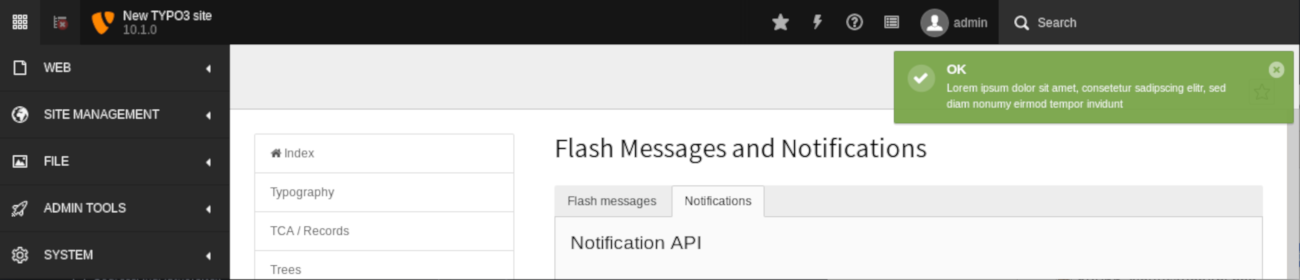
\includegraphics[width=0.90\linewidth]{ChangesForDevelopers/89066-NotificationApi.png}
%	\end{figure}
%
%\end{frame}

% ------------------------------------------------------------------------------
% Feature | 89061 | Introduce Notification Actions

\begin{frame}[fragile]
	\frametitle{Changements en profondeur}
	\framesubtitle{Actions dans les notifications}

	\begin{itemize}
		\item En backend, les notifications JavaScript supportent l'usage d'actions (boutons).
	\end{itemize}

	\begin{figure}
		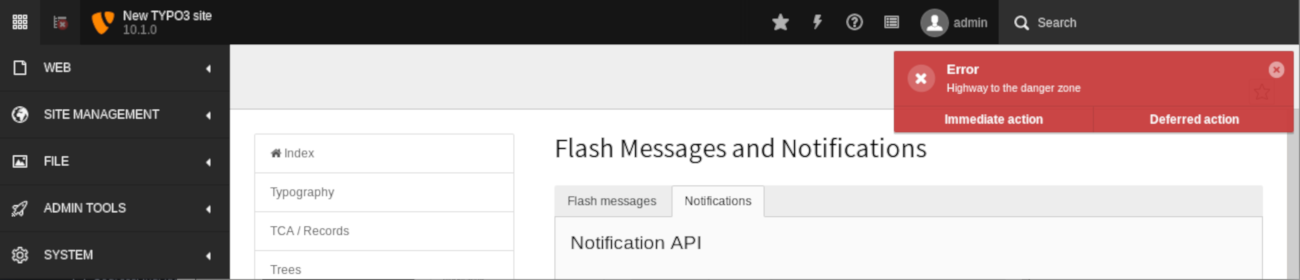
\includegraphics[width=0.90\linewidth]{InDepthChanges/89061-NotificationActionsAndButtons.png}
	\end{figure}

\end{frame}

% ------------------------------------------------------------------------------
% Feature | 89244 | Broadcast Channels and Messaging

\begin{frame}[fragile]
	\frametitle{Changements en profondeur}
	\framesubtitle{Canaux de diffusion et messages (1)}

	% decrease font size for code listing
	\lstset{basicstyle=\tiny\ttfamily}

	\begin{itemize}
		\item Il est possible de transmettre et recevoir des messages en JavaScript.
	\end{itemize}

	\vspace{-0.2cm}
	\begingroup
		\color{red}
			\begin{center}
				L'API est considérée \textbf{interne} pour le moment\newline
				et peut changer jusqu'à qu'elle soit déclarée «~stable~».
			\end{center}
	\endgroup

	\begin{itemize}
		\item Exemple pour \textbf{transmettre} un message~:
\begin{lstlisting}
require(['TYPO3/CMS/Backend/BroadcastService'], function (BroadcastService) {
  const payload = {
    componentName: 'my_extension',
    eventName: 'my_event',
    foo: 'bar'
  };
  BroadcastService.post(payload);
});
\end{lstlisting}

	\end{itemize}

\end{frame}

% ------------------------------------------------------------------------------
% Feature | 89244 | Broadcast Channels and Messaging

\begin{frame}[fragile]
	\frametitle{Changements en profondeur}
	\framesubtitle{Canaux de diffusion et messages (2)}

	% decrease font size for code listing
	\lstset{basicstyle=\tiny\ttfamily}

	\begin{itemize}
		\item Exemple pour \textbf{recevoir} le message~:
\begin{lstlisting}
define([], function() {
  document.addEventListener('typo3:my_component:my_event', (e) => eventHandler(e.detail));
  function eventHandler(detail) {
    // output contains key 'foo' as the payload
    console.log(detail);
  }
});
\end{lstlisting}

		\item Voir \href{https://developer.mozilla.org/en-US/docs/Web/API/Broadcast_Channel_API}{developer.mozilla.org (en)}
			pour plus d'informations.

	\end{itemize}

\end{frame}

% ------------------------------------------------------------------------------
% Feature | 88871 | Handle middleware handler in RequestFactory correctly

\begin{frame}[fragile]
	\frametitle{Changements en profondeur}
	\framesubtitle{Gestionnaire Middleware de RequestFactory}

	% decrease font size for code listing
	\lstset{basicstyle=\tiny\ttfamily}

	\begin{itemize}
		\item Il est possible de définir la liste des gestionnaires middleware.
		\item RequestFactory construire une pile de gestionnaires basé sur\newline
			\small
				\texttt{\$GLOBALS['TYPO3\_CONF\_VARS']['HTTP']['handler']}
			\normalsize
			et l'injecte dans le client.
		\item Par exemple~:
\begin{lstlisting}
use \TYPO3\CMS\Core\Utility\GeneralUtility;
use \Vendor\MyExtension\Middleware\Guzzle\CustomMiddleware;
use \Vendor\MyExtension\Middleware\Guzzle\SecondCustomMiddleware;

# Add custom middleware to default Guzzle handler stack
\$GLOBALS['TYPO3_CONF_VARS']['HTTP']['handler'][] =
  (GeneralUtility::makeInstance(CustomMiddleware::class))->handler();
\$GLOBALS['TYPO3_CONF_VARS']['HTTP']['handler'][] =
  (GeneralUtility::makeInstance(SecondCustomMiddleware::class))->handler();
\end{lstlisting}

	\end{itemize}

\end{frame}

% ------------------------------------------------------------------------------
% Feature | 88602 | Allow registering additional file processors

\begin{frame}[fragile]
	\frametitle{Changements en profondeur}
	\framesubtitle{Processeurs de fichier personnalisés}

	% decrease font size for code listing
	\lstset{basicstyle=\tiny\ttfamily}

	\begin{itemize}
		\item Les développeurs peuvent inscrire leur propre processeurs de fichiers.
		\item Ajouter le code suivant au fichier \texttt{ext\_localconf.php}~:
\begin{lstlisting}
\$GLOBALS['TYPO3_CONF_VARS']['SYS']['fal']['processors']['ExampleImageProcessor'] = [
  'className' => \Vendor\MyExtension\Resource\Processing\ExampleImageProcessor::class,
  'before' => 'LocalImageProcessor',
];
\end{lstlisting}

		\item Cas d'usage typiques~:

			\begin{itemize}
				\item Ajouter un filigrane aux images
				\item Compresser les fichiers envoyés dans une archive ZIP
				\item Enregistrer les versions modifiées des images
				\item etc.
			\end{itemize}

	\end{itemize}

\end{frame}

% ------------------------------------------------------------------------------
% Feature | 88950 | Add storeSession argument to Widget ViewHelpers

\begin{frame}[fragile]
	\frametitle{Changements en profondeur}
	\framesubtitle{Widget ViewHelpers}

	% decrease font size for code listing
	\lstset{basicstyle=\smaller\ttfamily}

	\begin{itemize}
		\item Les Widget ViewHelpers posent un cookie de session frontend dans certaines conditions.
		\item Comme ce n'est pas toujours souhaité (par exemple en raison de RGPD), c'est contrôlable.
		\item Un booléen \texttt{storeSession} est introduit permettant au développeur de contrôler cette fonction.
\begin{lstlisting}
<f:widget.autocomplete
  for="name"
  objects="{posts}"
  searchProperty="author"
  storeSession="false" />
\end{lstlisting}

	\end{itemize}

\end{frame}

% ------------------------------------------------------------------------------
% Feature | 89577 | New PSR-14 based events for File Abstraction Layer
% Deprecation | 89577 | FAL SignalSlot handling migrated to PSR-14 events

\begin{frame}[fragile]
	\frametitle{Changements en profondeur}
	\framesubtitle{Événements PSR-14 dans FAL}

	% decrease font size for code listing
	\lstset{basicstyle=\tiny\ttfamily}

	\begin{itemize}
		\item Environ 40 nouveaux événements basés sur
			\href{https://www.php-fig.org/psr/psr-14/}{PSR-14}
			sont introduits dans la couche d'abstraction des fichiers (FAL).
		\item Ils remplacent les Signal/Slots extbase existants.
		\item Les Signals sont toujours fonctionnels (sans message de dépréciation).
			Cependant, ces derniers sont susceptibles d'être retirés dans TYPO3 v11.
		\item Il est conseillé aux auteurs d'extension de migrer leur code et utiliser ces événements.
		\item Consultez les nouvelles classes PHP pour en savoir plus sur PSR-14.
	\end{itemize}

\end{frame}


% ------------------------------------------------------------------------------
% Deprecation | 89733 | Signal Slots in Core Extension migrated to PSR-14 events

\begin{frame}[fragile]
	\frametitle{Changements en profondeur}
	\framesubtitle{Événements PSR-14 dans le noyau TYPO3}

	\begin{itemize}
		\item Des événements PSR-14 remplacent les Signal/Slots dans le noyau TYPO3~:
			\newline

			\begin{itemize}\tiny
				\item \texttt{TYPO3\textbackslash
					CMS\textbackslash
					Core\textbackslash
					Imaging\textbackslash
					Event\textbackslash
					ModifyIconForResourcePropertiesEvent}
					\newline
				\item \texttt{TYPO3\textbackslash
					CMS\textbackslash
					Core\textbackslash
					DataHandling\textbackslash
					Event\textbackslash
					IsTableExcludedFromReferenceIndexEvent}
					\newline
				\item \texttt{TYPO3\textbackslash
					CMS\textbackslash
					Core\textbackslash
					DataHandling\textbackslash
					Event\textbackslash
					AppendLinkHandlerElementsEvent}
					\newline
				\item \texttt{TYPO3\textbackslash
					CMS\textbackslash
					Core\textbackslash
					Configuration\textbackslash
					Event\textbackslash
					AfterTcaCompilationEvent}
					\newline
				\item \texttt{TYPO3\textbackslash
					CMS\textbackslash
					Core\textbackslash
					Database\textbackslash
					Event\textbackslash
					AlterTableDefinitionStatementsEvent}
					\newline
				\item \texttt{TYPO3\textbackslash
					CMS\textbackslash
					Core\textbackslash
					Tree\textbackslash
					Event\textbackslash
					ModifyTreeDataEvent}
					\newline
				\item \texttt{TYPO3\textbackslash
					CMS\textbackslash
					Backend\textbackslash
					Backend\textbackslash
					Event\textbackslash
					SystemInformationToolbarCollectorEvent}
					\newline
			\end{itemize}

	\end{itemize}

\end{frame}

% ------------------------------------------------------------------------------
% Deprecation | 89718 | Legacy PageTSconfig parsing lowlevel API

\begin{frame}[fragile]
	\frametitle{Changements en profondeur}
	\framesubtitle{Traitement du TSconfig}

	% decrease font size for code listing
	\lstset{basicstyle=\tiny\ttfamily}

	\begin{itemize}
		\item Deux classes sont introduites pour charger et traiter le TSconfig de page~:
			\begin{itemize}\smaller
				\item \texttt{TYPO3\textbackslash
					CMS\textbackslash
					Core\textbackslash
					Configuration\textbackslash
					Loader\textbackslash
					PageTsConfigLoader}
				\item \texttt{TYPO3\textbackslash
					CMS\textbackslash
					Core\textbackslash
					Configuration\textbackslash
					Parser\textbackslash
					PageTsConfigParser}
			\end{itemize}

		\item Par exemple~:
\begin{lstlisting}
// Fetch all available PageTS of a page/rootline:
\$loader = GeneralUtility::makeInstance(PageTsConfigLoader::class);
\$tsConfigString = \$loader->load(\$rootLine);

// Parse the string and apply conditions:
\$parser = GeneralUtility::makeInstance(
  PageTsConfigParser::class, \$typoScriptParser, \$hashCache
);

\$pagesTSconfig = \$parser->parse(\$tsConfigString, \$conditionMatcher);
\end{lstlisting}

	\end{itemize}

\end{frame}

% ------------------------------------------------------------------------------
% Important | 87518 | Use prepared statements for pdo_mysql per default

\begin{frame}[fragile]
	\frametitle{Changements en profondeur}
	\framesubtitle{Prepared Statements}

	% decrease font size for code listing
	\lstset{basicstyle=\tiny\ttfamily}

	\begin{itemize}
		\item Le pilote \texttt{pdo\_mysql} utilise les prepared statements par défaut.
		\item Dans les anciennes versions de TYPO3, des \textit{prepared statements émulés} sont utilisés.
			En conséquence, les valeurs retournées par les requêtes étaient des chaînes de caractères.
		\item Ce comportement est changé et les prepared statements sont utilisés,
			retournant les types de donnée natifs.
		\item Par exemple~: les valeurs d'une colonne définie comme entier sont retournés en PHP comme \texttt{int}.
		\item La fonctionnalité est désactivable en ajoutant l'option
			\texttt{PDO::ATTR\_EMULATE\_PREPARES} à votre connexion à la base de données.

	\end{itemize}

\end{frame}

% ------------------------------------------------------------------------------
% Feature | 87380 | Introduce SiteLanguageAwareInterface to denote site language awareness

\begin{frame}[fragile]
	\frametitle{Changements en profondeur}
	\framesubtitle{Signifier la prise en charge de la langue de site}

	% decrease font size for code listing
	\lstset{basicstyle=\tiny\ttfamily}

% A SiteLanguageAwareInterface with the methods setSiteLanguage(Entity\SiteLanguage $siteLanguage) and getSiteLanguage() has been introduced.
% The interface can be used to denote a class as aware of the site language.

	\begin{itemize}
		\item L'interface \texttt{SiteLanguageAwareInterface} est introduite.
		\item Celle-ci permet de signifier qu'un classe prend en charge la langue du site.
		\item Les extensions du routage, qui prennent en compte la langue du site,
			utilisent donc \texttt{SiteLanguageAwareInterface}
			en plus de \texttt{SiteLanguageAwareTrait}.
	\end{itemize}

\end{frame}

% ------------------------------------------------------------------------------
% Important | 89645 | Removed systemLog options

\begin{frame}[fragile]
	\frametitle{Changements en profondeur}
	\framesubtitle{API de journalisation système}

	% decrease font size for code listing
	\lstset{basicstyle=\tiny\ttfamily}

	\begin{itemize}
		\item Les options de configurations suivantes sont retirées de la configuration par défaut~:

			\begin{itemize}\smaller
				\item \texttt{\$GLOBALS['TYPO3\_CONF\_VARS']['SYS']['systemLog']}
				\item \texttt{\$GLOBALS['TYPO3\_CONF\_VARS']['SYS']['systemLogLevel']}
			\end{itemize}\normalsize

		\item Il est conseillé aux auteurs d'extension d'utiliser l'API de journalisation et de retirer
			l'option systemLog.
	\end{itemize}

\end{frame}

% ------------------------------------------------------------------------------
% Feature | 89603 | Introduce native pagination for lists

\begin{frame}[fragile]
	\frametitle{Changements en profondeur}
	\framesubtitle{Pagination native de listes}

	% decrease font size for code listing
	\lstset{basicstyle=\tiny\ttfamily}

	\begin{itemize}
		\item Le support natif de la pagination de listes comme les tableaux ou
			les résultats de requête Extbase est introduit.
		\item La \texttt{PaginatorInterface} définie le jeu de méthodes de base.
		\item La classe \texttt{AbstractPaginator} contient la logique de pagination principale.
		\item Les développeurs peuvent donc implémenter de nouvelles paginations.
\begin{lstlisting}
use TYPO3\CMS\Core\Pagination\ArrayPaginator;

\$items = ['apple', 'banana', 'strawberry', 'raspberry', 'ananas'];
\$currentPageNumber = 3;
\$itemsPerPage = 2;

\$paginator = new ArrayPaginator(\$itemsToBePaginated, \$currentPageNumber, \$itemsPerPage);
\$paginator->getNumberOfPages(); // returns 3
\$paginator->getCurrentPageNumber(); // returns 3
\$paginator->getKeyOfFirstPaginatedItem(); // returns 5
\$paginator->getKeyOfLastPaginatedItem(); // returns 5
\end{lstlisting}

	\end{itemize}

\end{frame}

% ------------------------------------------------------------------------------
% Deprecation | 89579 | ServiceChains require an array for excluded Service keys

\begin{frame}[fragile]
	\frametitle{Changements en profondeur}
	\framesubtitle{API des services}

	\begin{itemize}
		\item L'argument \texttt{\$excludeServiceKeys} est utilisé pour ignorer certains services lors l'utilisation
			d'une séquence de services.
		\item Le format de l'argument est changé de liste séparée par la virgule en tableau.
		\item Ce changement impacte l'API des services dans ces composants~:

			\begin{itemize}
				\item \texttt{GeneralUtility::makeInstanceService()}
				\item \texttt{ExtensionManagementUtility::findService()}
			\end{itemize}

		\item Passer l'ancien format fonctionne toujours mais est marqué \textbf{déprécié}.

	\end{itemize}

\end{frame}

% ------------------------------------------------------------------------------
% Feature | 86614 | Add PSR-14 event to control hreflang tags to be rendered

\begin{frame}[fragile]
	\frametitle{Changements en profondeur}
	\framesubtitle{Modifier les balises \texttt{hreflang}}

	% decrease font size for code listing
	\lstset{basicstyle=\smaller\ttfamily}

	\begin{itemize}
		\item Il est possible d'altérer les balises \texttt{hreflang} avant qu'elles soient transmises.
		\item Il faut inscrire un écouteur à l'événement suivant~:\newline
			\smaller
				\texttt{TYPO3\textbackslash
					CMS\textbackslash
					Frontend\textbackslash
					Event\textbackslash
					ModifyHrefLangTagsEvent}
			\normalsize
	\end{itemize}

\end{frame}

% ------------------------------------------------------------------------------
% Feature | 88818 | Introduce events to modify CKEditor configuration

\begin{frame}[fragile]
	\frametitle{Changements en profondeur}
	\framesubtitle{Modifier la configuration de CKEditor}

	% decrease font size for code listing
	\lstset{basicstyle=\tiny\ttfamily}

	\begin{itemize}
		\item Les événements basés sur PSR-14 suivants permettent d'altérer la configuration de CKEditor~:
\begin{lstlisting}
TYPO3\CMS\RteCKEditor\Form\Element\Event\AfterGetExternalPluginsEvent
TYPO3\CMS\RteCKEditor\Form\Element\Event\BeforeGetExternalPluginsEvent
TYPO3\CMS\RteCKEditor\Form\Element\Event\AfterPrepareConfigurationForEditorEvent
TYPO3\CMS\RteCKEditor\Form\Element\Event\BeforePrepareConfigurationForEditorEvent
\end{lstlisting}

		\item Voir le
			\href{https://docs.typo3.org/c/typo3/cms-core/master/en-us/Changelog/10.3/Feature-88818-IntroduceEventsToModifyCKEditorConfiguration.html}{journal des modifications (en)}
			pour un exemple.
	\end{itemize}

\end{frame}

% ------------------------------------------------------------------------------
% Feature | 89738 | API for AJAX Requests

\begin{frame}[fragile]
	\frametitle{Changements en profondeur}
	\framesubtitle{API pour les requêtes AJAX}

	% decrease font size for code listing
	\lstset{basicstyle=\tiny\ttfamily}

	\begin{itemize}
		\item L'API \textbf{Fetch} est introduite pour effectuer des requêtes AJAX
			et pour rendre TYPO3 moins dépendant de jQuery.
		\item L'API fournit une définition générique d'objets Requête et Réponse
			(et d'autres éléments impliqués dans les requêtes réseau)
		\item Supportée par tous les navigateurs modernes, voir le
			\href{https://developer.mozilla.org/en-US/docs/Web/API/Fetch_API}{tableau de compatibilité (en)}.
		\item Le noyau de TYPO3 utilise déjà la nouvelle API dans l'outils d'installation, le moteur de
			formulaire et les menus contextuels.
		\item Voir le
			\href{https://docs.typo3.org/c/typo3/cms-core/master/en-us/Changelog/10.3/Feature-89738-ApiForAjaxRequests.html}{journal des modifications (en)}
			pour des exemples de comment utiliser l'API Fetch.

	\end{itemize}

\end{frame}

% ------------------------------------------------------------------------------
% Feature | 89650 | Allow line breaks in TCA descriptions

\begin{frame}[fragile]
	\frametitle{Changements en profondeur}
	\framesubtitle{Champs de description TCA}

	\begin{itemize}
		\item Les sauts de ligne sont acceptés dans les champs de description TCA
			pour rendre les texte longs plus lisibles.
	\end{itemize}

\end{frame}

% ------------------------------------------------------------------------------
% Important | 90020 | Legacy BasicFileUtility and ExtendedFileUtility classes marked as internal

\begin{frame}[fragile]
	\frametitle{Changements en profondeur}
	\framesubtitle{Classes \texttt{BasicFileUtility} et \texttt{ExtendedFileUtility}}

	\begin{itemize}
		\item Ces deux anciennes classes sont marquées \textbf{internes}
			et ne doivent plus être utilisées~:

			\begin{itemize}\small
				\item \texttt{TYPO3\textbackslash
					CMS\textbackslash
					Core\textbackslash
					Utility\textbackslash
					File\textbackslash
					BasicFileUtility}
				\item \texttt{TYPO3\textbackslash
					CMS\textbackslash
					Core\textbackslash
					Utility\textbackslash
					File\textbackslash
					ExtendedFileUtility}
			\end{itemize}

		\item Les développeurs doivent utiliser les classes \texttt{ResourceStorage}
			et \texttt{ResourceFactory} pour gérer les fichiers.

	\end{itemize}

\end{frame}

% ------------------------------------------------------------------------------
% Feature | 89139 | Add dependency injection support for console commands

\begin{frame}[fragile]
	\frametitle{Changements en profondeur}
	\framesubtitle{Commandes de Console~: Support Symfony DI}

	\begin{itemize}
		\item Les dépendances des commandes peuvent être injectées par le constructeur ou d'autres
			techniques d'injection.
		\item Ajoutez la balise \texttt{console.command} aux classes de commande.
		\item Utilisez la balise d'attribut \texttt{command} pour spécifier le nom de la commande.
		\item Pour exclure la commande du planificateur TYPO3, il faut définir la balise d'attribut
			optionnel \texttt{schedulable} à \texttt{false}.

		\item Voir le
			\href{https://docs.typo3.org/c/typo3/cms-core/master/en-us/Changelog/10.3/Feature-89139-AddDependencyInjectionSupportForConsoleCommands.html}{journal des modifications (en)}
			pour un exemple.
	\end{itemize}

\end{frame}

% ------------------------------------------------------------------------------
% Feature | 90168 | Introduce Modal Actions

\begin{frame}[fragile]
	\frametitle{Changements en profondeur}
	\framesubtitle{Boutons d'action dans les boîtes de dialogue}

	% decrease font size for code listing
	\lstset{basicstyle=\tiny\ttfamily}

	\begin{itemize}
		\item Les boîtes de dialogue supportent les boutons d'action.
		\item En alternative à l'option existante \texttt{trigger}, la nouvelle
			option \texttt{action} est disponible.
		\item Par exemple~:
\begin{lstlisting}
Modal.confirm('Header', 'Some content', Severity.error, [
  {
    text: 'Based on trigger()',
    trigger: function () {
      console.log('Vintage!');
    }
  },
  {
    text: 'Based on action()',
    action: new DeferredAction(() => {
      return new AjaxRequest('/any/endpoint').post({});
    })
  }
]);
\end{lstlisting}

	\end{itemize}

\end{frame}

% ------------------------------------------------------------------------------
% Feature | 90471 | JavaScript Event API

\begin{frame}[fragile]
	\frametitle{Changements en profondeur}
	\framesubtitle{API d'événement JavaScript}

	\begin{itemize}
		\item L'API d'Événement JavaScript permet aux développeurs d'avoir une
			interface d'écoute d'événement stable.
		\item L'API prend en charge les écueils habituels comme la délégation
			d'événement et le détachement propre d'événement.
		\item Chaque \textit{event strategy} offre deux manières d'associer un
			écouteur à un événement
		\item L'API d'Événement offres plusieurs stratégies pour gérer les écouteurs.
		\item Voir le
			\href{https://docs.typo3.org/c/typo3/cms-core/master/en-us/Changelog/10.3/Feature-90471-JavaScriptEventAPI.html}{journal des modifications (en)}
			pour des exemples et plus de détails.
	\end{itemize}

\end{frame}

% ------------------------------------------------------------------------------
% Feature | 88648 | Define Twitter Card Type In Page Properties
% Important | 86577 | Query parameters are now included in canonicalized URLs

\begin{frame}[fragile]
	\frametitle{Changements en profondeur}
	\framesubtitle{Divers (1)}

	% decrease font size for code listing
	\lstset{basicstyle=\tiny\ttfamily}

	\begin{itemize}

		\item Le type de Twitter Card est configurable.
			Cette option agit sur le rendu de la métadonnée \texttt{twitter:card} en FrontEnd.
\begin{lstlisting}
page {
  meta {
    twitter:card = summary_large_image
    twitter:card.replace = 1
  }
}
\end{lstlisting}

		\item Seuls les paramètres nécessaires pour le calcul du cHash sont inclus dans les URLs canoniques par défaut.
			Des paramètres de requête additionnels peuvent être configurés~:
\begin{lstlisting}
\$GLOBALS['TYPO3_CONF_VARS']['FE']['additionalCanonicalizedUrlParameters'].
\end{lstlisting}

		\smaller
			Remarque~: N'ajoutez que les paramètres qui changent le contenu de la page. Dans le cas contraire les
			moteurs de recherche risquent de classifier vos pages en contenu dupliqué.
		\normalsize

	\end{itemize}

\end{frame}

% ------------------------------------------------------------------------------
% Breaking | 88681 | Import Of PHP Files In Import Export Files Removed
% Breaking | 88500 | RTE image handling functionality dropped
% Breaking | 81950 | Remove leftover workspaces unpublishing functionality

\begin{frame}[fragile]
	\frametitle{Changements en profondeur}
	\framesubtitle{Divers (2)}

	% decrease font size for code listing
	\lstset{basicstyle=\tiny\ttfamily}

	\begin{itemize}

		\item Lors de l'import de données XML de \texttt{EXT:impexp}, les motifs d'exclusion de
			fichier s'appliquent et rejettent en autres les fichiers PHP encapsulés.

		\item La gestion des images dans le RTE est intégralement retirée.
			Pour le support des images dans CKEditor, utilisez l'extension \texttt{EXT:rte\_ckeditor\_image} par exemple.

		\item Une propriété des espaces de travail pour dépublier les enregistrements est retirée de TYPO3 v10
			(y compris le champ de base de données \texttt{sys\_workspace.unpublish\_time}).
			Cette fonctionnalité fut désactivée dans TYPO3 v4.5 et n'est plus utilisée ou fournie depuis.

	\end{itemize}

\end{frame}

% ------------------------------------------------------------------------------
% Breaking | 88772 | JavaScript script tags omit type=text/javascript in HTML5
% Remove system extension EXT:rsaauth
% Remove system extension EXT:fe_edit

\begin{frame}[fragile]
	\frametitle{Changements en profondeur}
	\framesubtitle{Divers (3)}

	% decrease font size for code listing
	\lstset{basicstyle=\tiny\ttfamily}

	\begin{itemize}

		\item Lors du rendu en HTML5, les balises \texttt{<script>} n'incluent plus l'attribut \texttt{type="text/javascript"}.
		\item Pour le réactiver en frontend, utilisez le TypoScript ci-dessous~:

\begin{lstlisting}
page {
  includeJS {
    myfile = EXT:example/Resources/Public/JavaScript/myfile.js
    myfile.type = text/javascript
  }
}
\end{lstlisting}

		\item Les extensions système dépréciées suivantes sont retirées~:
			\begin{itemize}
				\item \texttt{EXT:rsaauth}
				\item \texttt{EXT:fe\_edit}
			\end{itemize}

	\end{itemize}

\end{frame}

% ------------------------------------------------------------------------------
% Breaking | 88525 | Remove “createDirs” directive of extension installation / ext_emconf.php
% Breaking | 87511 | Remove $viewFormatToObjectNameMap property
% Breaking | 87511 | Remove $namespacesViewObjectNamePattern property
% Feature | 87726 | Extend Frontend Login Controller Hook To Validate Password

\begin{frame}[fragile]
	\frametitle{Changements en profondeur}
	\framesubtitle{Divers (4)}

	\begin{itemize}
		\item La directive \texttt{createDirs} du fichier \texttt{ext\_emconf.php} n'est plus supportée.

			\begin{itemize}\smaller
				\item[\ding{228}] Les dossiers ne sont plus créés automatiquement au cours de l'installation d'une extension.
			\end{itemize}\normalsize

		\item Ces deux propriétés de la classe
			\texttt{TYPO3\textbackslash
				CMS\textbackslash
				Extbase\textbackslash
				Mvc\textbackslash
				Controller\textbackslash
				ActionController}\newline
			sont retirées~:

			\begin{itemize}
				\item \texttt{\$namespacesViewObjectNamePattern}
				\item \texttt{\$viewFormatToObjectNameMap}
			\end{itemize}

		\item Le hook suivant est étendu et permet aussi d'être utilisé pour la validation des mots de passe~:\newline
			{\fontsize{8}{10} \selectfont \texttt{\$GLOBALS['TYPO3\_CONF\_VARS']['EXTCONF']['felogin']['password\_changed']}}

	\end{itemize}

\end{frame}

% ------------------------------------------------------------------------------
% Deprecation | 87613 | Deprecate /TYPO3/CMS/Extbase/Utility/TypeHandlingUtility::hex2bin
% Deprecation | 88554 | Deprecated methods in VersionNumberUtility

\begin{frame}[fragile]
	\frametitle{Changements en profondeur}
	\framesubtitle{Divers (5)}

	\begin{itemize}

		\item La méthode suivante est dépréciée~:\newline
			\smaller\texttt{\textbackslash
				TYPO3\textbackslash
				CMS\textbackslash
				Extbase\textbackslash
				Utility\textbackslash
				TypeHandlingUtility::hex2bin()}\normalsize

			\begin{itemize}\smaller
				\item[\ding{228}] Utilisez la fonction native PHP \href{https://www.php.net/manual/en/function.hex2bin.php}{hex2bin()}
			\end{itemize}\normalsize

		\item Les méthodes suivantes de la classe
			\smaller\texttt{\textbackslash
				TYPO3\textbackslash
				CMS\textbackslash
				Core\textbackslash
				Utility\textbackslash
				VersionNumberUtility}\normalsize\newline
			sont marquées dépréciées~:

			\begin{itemize}
				\item \texttt{convertIntegerToVersionNumber()}
				\item \texttt{splitVersionRange()}
				\item \texttt{raiseVersionNumber()}
			\end{itemize}

			\begin{itemize}\smaller
				\item[\ding{228}] Implémentez la méthode dans votre code.
			\end{itemize}\normalsize

	\end{itemize}

\end{frame}

% ------------------------------------------------------------------------------
% Feature | 86964 | Allow getting class property default value
% Deprecation | 82669 | Streamline Backend route path inconsistencies

\begin{frame}[fragile]
	\frametitle{Changements en profondeur}
	\framesubtitle{Divers (6)}

	% decrease font size for code listing
	\lstset{basicstyle=\tiny\ttfamily}

	\begin{itemize}
		\item La valeur par défaut d'une propriété de classe est récupérable avec le service de réflexion.
\begin{lstlisting}
\$property = GeneralUtility::makeInstance(ReflectionService::class)
  ->getClassSchema(MyClass::class)
  ->getProperty('myProperty');
\end{lstlisting}

		\item Les routes backend vers les modules n'ayant pas de configuration de chemin sont nommées\newline
			«~\texttt{/module/<main-module>/<sub-module>}~» par défaut\newline
			\small
				(par exemple~: «~\texttt{/module/web/ts}~».)
			\normalsize

		\item Les anciennes routes fonctionnent toujours (i.e. «~\texttt{/web/ts/}~») mais la syntaxe sera
			enlevée de TYPO3 v11.

	\end{itemize}

\end{frame}

% ------------------------------------------------------------------------------
% Breaking | 88669 | FormEngine FormDataProvider parentPageTca removed
% Breaking | 88744 | Database fields related to CSS Styled Content removed
% Breaking | 88143 | Version-related database field “t3ver_id” removed
% Deprecation | 88746 | PageRepository PHP class moved from Frontend to Core Extension

\begin{frame}[fragile]
	\frametitle{Changements en profondeur}
	\framesubtitle{Divers (7)}

	\begin{itemize}
		\item La clé \texttt{parentPageTca} est retirée du fournisseur de données de FormEngine.

			\begin{itemize}\smaller
				\item[\ding{228}] Les développeurs peuvent accéder à \texttt{\$GLOBALS['TCA']['pages']} directement,
					en lieu et place de \texttt{\$result['parentPageTca']}.
			\end{itemize}\normalsize

		\item Les champs de base suivants sont retirés~:

			\begin{itemize}\smaller
				\item \texttt{tt\_content.spaceBefore} (remplacé par \texttt{space\_before\_class})
				\item \texttt{tt\_content.spaceAfter} (remplacé par \texttt{space\_after\_class})
				\item \texttt{pages.t3ver\_id} (inutilisé depuis TYPO3 v9)
			\end{itemize}\normalsize

		\item La classe PHP
			\texttt{\textbackslash
				TYPO3\textbackslash
				CMS\textbackslash
				Frontend\textbackslash
				Page\textbackslash
				PageRepository} est déplacé de l'extension système frontend vers le cœur.

			\begin{itemize}\smaller
				\item Remplacez par la classe~:
					\texttt{\textbackslash
						TYPO3\textbackslash
						CMS\textbackslash
						Core\textbackslash
						Domain\textbackslash
						Repository\textbackslash
						PageRepository}
			\end{itemize}\normalsize

	\end{itemize}

\end{frame}

% ------------------------------------------------------------------------------
% Breaking | 88574 | 4th parameter of PageRepository>enableFields removed
% Deprecation | 85895 | Deprecate File::_getMetaData()
% Deprecation | 88662 | Deprecated backend route xMOD_tximpexp

\begin{frame}[fragile]
	\frametitle{Changements en profondeur}
	\framesubtitle{Divers (8)}

	\begin{itemize}

		\item Le 4ième paramètre de la méthode \texttt{PageRepository->enableFields()} est retiré.

		\begin{itemize}\smaller
			\item[\ding{228}] Si les développeurs utilisent un 4ème paramètre dans cet appel de méthode,
				mis à «~\textbf{false}~», il est sûr de le retirer.
			\item[\ding{228}] S'il est paramétré à «~\textbf{true}~», le code doit être remplacé par une
				instance séparée de \texttt{PageRepository} avec un paramètre \texttt{Context} adapté.
		\end{itemize}\normalsize

		\item La méthode interne \texttt{File::\_getMetaData()}, utilisée pour la récupération des
			métadonnées d'un fichier est marquée dépréciée.

			\begin{itemize}\smaller
				\item[\ding{228}] Utilisez plutôt \texttt{\$fileObject->getMetaData()->get()} pour la récupération de métadonnées.
			\end{itemize}\normalsize

		\item L'identifiant de route «~\texttt{xMOD\_tximpexp}~» est marqué déprécié.

			\begin{itemize}\smaller
				\item[\ding{228}] Utilisez \texttt{tx\_impexp\_export} ou \texttt{tx\_impexp\_import} selon le cas.
			\end{itemize}\normalsize

	\end{itemize}

\end{frame}

% ------------------------------------------------------------------------------
% Breaking | 88496 | Method getSwitchableControllerActions has been removed
% Breaking | 87567 | Global variable $TBE_TEMPLATE removed
% Breaking | 88660 | $GLOBALS[T3_VAR] removed

\begin{frame}[fragile]
	\frametitle{Changements en profondeur}
	\framesubtitle{Divers (9)}

	\begin{itemize}

		\item La méthode abstraite suivante est retirée~:\newline
			\smaller
				\texttt{\textbackslash
					TYPO3\textbackslash
					CMS\textbackslash
					Extbase\textbackslash
					Configuration\textbackslash
					AbstractConfigurationManager::}\newline
					\texttt{getSwitchableControllerActions()}
			\normalsize

			\begin{itemize}\smaller
				\item[\ding{228}] Utilisez le nouveau nom de méthode \texttt{getControllerConfiguration()} (même classe PHP)
			\end{itemize}\normalsize

		\item La variable globale \texttt{\$TBE\_TEMPLATE} est retirée, avec le middleware PSR-15 lié (qui était marqué comme interne).

			\begin{itemize}\smaller
				\item[\ding{228}] Instanciez la classe DocumentTemplate directement dans le contrôleur du module.
				\item[\ding{228}] Migrez vers le ModuleTemplate (disponible depuis TYPO3 v7).
			\end{itemize}\normalsize

		\item La variable globale \texttt{\$GLOBALS['T3\_VAR']} est retirée.\newline

	\end{itemize}

\end{frame}

% ------------------------------------------------------------------------------
% Important | 89001 | TSFE->createHashBase
% Feature | 89150 | Add events before and after rollback of record history entries

\begin{frame}[fragile]
	\frametitle{Changements en profondeur}
	\framesubtitle{Divers (10)}

	\begin{itemize}
		\item Les paramètres de base utilisés pour calculer les signatures de cache sont
			modifiés dans la classe~:\newline
			\small
				\texttt{TYPO3\textbackslash
					CMS\textbackslash
					Frontend\textbackslash
					Controller\textbackslash
					TypoScriptFrontendController}
			\normalsize

			\begin{itemize}
				\item \texttt{gr\_list} est remplacé par \texttt{groupIds}.
				\item \texttt{cHash} est remplacé par \texttt{dynamicArguments}.
				\item \texttt{domainStartPage} est remplacé par \texttt{site} (identifiant du site).
			\end{itemize}

		\item Deux événements sont déclenchés lors d'un retour arrière d'un enregistrements~:

			\begin{itemize}\smaller
				\item \texttt{TYPO3\textbackslash
					CMS\textbackslash
					Backend\textbackslash
					History\textbackslash
					Event\textbackslash
					BeforeHistoryRollbackStartEvent}
				\item \texttt{TYPO3\textbackslash
					CMS\textbackslash
					Backend\textbackslash
					History\textbackslash
					Event\textbackslash
					AfterHistoryRollbackFinishedEvent}
			\end{itemize}\normalsize

	\end{itemize}

\end{frame}

% ------------------------------------------------------------------------------
% Feature | 88805 | Add type to TYPO3/CMS/Core/Database/Query/QueryBuilder::set()

\begin{frame}[fragile]
	\frametitle{Changements en profondeur}
	\framesubtitle{Divers (11)}

	\begin{itemize}
		\item La méthode \texttt{set()} du générateur de requêtes accepte un 4ième argument
			pour spécifier le type du paramètre nommé~:\newline
			\small
				\texttt{TYPO3\textbackslash
					CMS\textbackslash
					Core\textbackslash
					Database\textbackslash
					Query\textbackslash
					QueryBuilder::set()}
			\normalsize\newline
			\vspace{0.2cm}
			(par défaut, c'est \texttt{\textbackslash PDO::PARAM\_STR})

	\end{itemize}

\end{frame}

% ------------------------------------------------------------------------------
% Feature | 21638 | Introduced IP locking for IPv6
% Breaking | 21638 | AbstractUserAuthentication::lockIP property removed

\begin{frame}[fragile]
	\frametitle{Changements en profondeur}
	\framesubtitle{Divers (12)}

	% decrease font size for code listing
	\lstset{basicstyle=\tiny\ttfamily}

	\begin{itemize}

		\item La fonctionnalité de verrouillage d'IP a été étendue pour supporter IPv6
			(frontend et backend).
\begin{lstlisting}
\$GLOBALS['TYPO3_CONF_VARS']['FE']['lockIPv6'] = 2;
\$GLOBALS['TYPO3_CONF_VARS']['BE']['lockIPv6'] = 2;
\end{lstlisting}

		\item La propriété publique \texttt{lockIP} dans la classe PHP suivante est retirée~:\newline
			\small
				\texttt{\textbackslash
					TYPO3\textbackslash
					CMS\textbackslash
					Core\textbackslash
					Authentication\textbackslash
					AbstractUserAuthentication}.
			\normalsize

		\item Options de migration~:

			\begin{itemize}\smaller
				\item[\ding{228}] Paramétrer \texttt{lockIP} et \texttt{lockIPv6} dans \texttt{\$GLOBALS['TYPO3\_CONF\_VARS'][\ldots]}.
				\item[\ding{228}] Utiliser la nouvelle API IP-Locker~:
					\texttt{\textbackslash
						TYPO3\textbackslash
						CMS\textbackslash
						Core\textbackslash
						Authentication\textbackslash
						IpLocker}.
			\end{itemize}\normalsize

	\end{itemize}

\end{frame}

% ------------------------------------------------------------------------------
